% =========================================================
% IIT BHUBANESWAR M.TECH LITERATURE SURVEY REPORT
% =========================================================

\documentclass[11pt,a4paper]{article}

\usepackage[utf8]{inputenc}
\usepackage[nottoc]{tocbibind}
\usepackage{amsmath,amssymb,amsfonts}
\usepackage{graphicx}
\usepackage{float}
\usepackage{caption}
\usepackage{subcaption}
\usepackage{array}
\usepackage{booktabs}
\usepackage{geometry}
\usepackage{xcolor}
\usepackage{setspace}
\usepackage{titlesec}
\usepackage{enumitem}
\usepackage{algorithm}
\usepackage{algpseudocode}
\algrenewcommand\algorithmicrequire{\textbf{Input:}}
\usepackage{hyperref}

\geometry{
left=2.2cm,
right=2.2cm,
top=2.2cm,
bottom=2.2cm
}

\hypersetup{
colorlinks=true,
linkcolor=blue,
citecolor=blue,
urlcolor=blue
}

\setstretch{1.2}

\titleformat{\section}
{\large\bfseries}
{\thesection.}{0.5em}{}

\titleformat{\subsection}
{\normalsize\bfseries}
{\thesubsection.}{0.5em}{}

\graphicspath{{figures/}}
\captionsetup{font=small,labelfont=bf}

\begin{document}

% =========================================================
% TITLE PAGE
% =========================================================

\begin{titlepage}

\begin{center}

\vspace*{1cm}

{\Huge \textbf{Rydberg Atomic Receivers for Future Wireless Communications}}\\[0.4cm]
\vspace{2em}
{\Large Report submitted as part of MTP Mid-Semester Evaluations}\\[0.2cm]
{\Large \textit{by}}\\[0.5cm]

{\LARGE \textbf{P SRIHARI}}\\[0.2cm]

{\Large Roll No: 25SP06015}\\[0.2cm]

{\Large M.Tech -- Signal Processing and Communications}\\[1.5cm]

{\Large \textit{Under the supervision of}}\\[0.3cm]

{\Large \textbf{Dr. Barathram Ramkumar}}\\
{\Large Associate Professor}\\[0.8cm]

{\Large \textit{Co-Supervisor}}\\[0.2cm]

{\Large \textbf{Dr. Soumya Prakash Dash}}\\
{\Large Associate Professor}\\[1.3cm]

\includegraphics[width=0.20\textwidth]{iitbbs.png}\\[0.8cm]

{\Large \textbf{School of Electrical Sciences}}\\[0.2cm]

{\Large \textbf{Indian Institute of Technology Bhubaneswar}}\\[0.2cm]

{\Large Odisha -- 752050}\\[1cm]


\end{center}

\end{titlepage}

% =========================================================
% CONTENTS
% =========================================================

\newpage

\tableofcontents

% =========================================================
% ABSTRACT
% =========================================================

\newpage

\section*{Abstract}
\addcontentsline{toc}{section}{Abstract}

Advances in quantum technology are opening new possibilities for sixth-generation (6G)
wireless communication. By exploiting the quantum properties of highly excited Rydberg atoms,
Rydberg atomic receivers offer clear advantages over conventional antennas, including very
high sensitivity, a wide operating frequency range and a compact size that does not depend on
the carrier wavelength. Since their use in communication systems has only recently begun,
suitable signal models and signal processing methods are still being developed. This report
presents the progress of the M.Tech project up to the mid-semester evaluation. A review of the
recent literature on Rydberg atomic receivers is presented, covering receiver models, atomic
multiple-input multiple-output (MIMO) detection and channel estimation. Two representative
works are then studied through simulation: the LO-free and LO-dressed receiver models are
implemented using a Lindblad master-equation solver (QuTiP), and channel estimation for one-
and two-dimensional atomic arrays is implemented in MATLAB. Based on this study, the research
directions for the remaining part of the project are identified.

% =========================================================
% 1. INTRODUCTION
% =========================================================

\newpage
\section{Introduction}

\subsection{Motivation}

In a conventional receiver the incoming electromagnetic (EM) wave induces a current in a
metal antenna, and this current is then amplified, filtered and down-converted by
electronic circuits. As explained in~\cite{cui2026rare}, this approach has three basic
limitations that become important for 6G systems.
\begin{enumerate}[leftmargin=*,itemsep=2pt]
  \item The antenna size must be of the order of the wavelength (about $\lambda/2$). Below
        $100$~MHz this means an antenna longer than $50$~cm.
  \item The amplifiers and mixers in the front-end add thermal noise ($-174$~dBm/Hz at room
        temperature), which fixes the minimum signal that can be detected.
  \item A resonant antenna works only around its design frequency, so separate antennas and
        RF chains are needed for sub-6~GHz, mmWave and THz bands.
\end{enumerate}

\subsection{Rydberg atomic receivers}

A Rydberg atom is an atom in which one electron is excited to a level with a large principal
quantum number ($n>20$). The size of such an atom grows as $n^2$, the gap between
neighbouring levels falls as $n^{-3}$ (which brings the transition frequencies into the
MHz--THz range), and the dipole moment becomes very large. Because of this, Rydberg atoms
react strongly even to weak RF fields.

In a Rydberg receiver, two lasers (probe and coupling) pass through a vapour cell and excite
the atoms to a Rydberg state, as illustrated in Fig.~\ref{fig:rare_setup}. The probe laser
takes the atoms from the ground state $|1\rangle$ to a low-excited state $|2\rangle$, and the
coupling laser takes them further to the Rydberg state $|3\rangle$. The RF signal couples this
Rydberg state to a neighbouring one, $|4\rangle$, and the effect is seen as a change in the
probe laser power measured by a photodetector (Section~\ref{sec:model}). The cell is roughly
$1~\text{cm}\times1~\text{mm}$ for any carrier frequency, it has no electronic front-end that
generates thermal noise, and it can be moved to a different band simply by choosing a
different pair of Rydberg levels~\cite{cui2026rare}.

\begin{figure}[H]
\centering
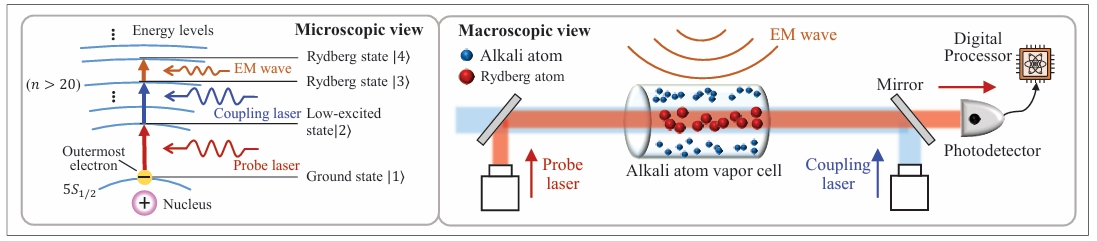
\includegraphics[width=\textwidth]{rare_setup.png}
\caption{Schematic of a Rydberg atomic receiver: four-level excitation scheme (left) and
vapour-cell setup with probe and coupling lasers and optical readout (right).
Adapted from~\cite{cui2026rare}.}
\label{fig:rare_setup}
\end{figure}

The use of these receivers in communication systems has only started recently, and the
existing papers model the receiver in two different ways. In the first, a local oscillator
(LO) is applied on the same Rydberg transition and the atoms behave like a mixer
(\textit{LO-dressed} or atomic-mixer
receiver)~\cite{chen2025harnessing,jing2020,simons2019}. In the second, a nearby reference
source adds to the user signals and only the magnitude of the total Rabi frequency is
measured, which leads to a phase-retrieval problem~\cite{cui2025towards,xu2025channel}.
This project considers both models and the signal processing required for each.

\subsection{Objectives}

\begin{enumerate}[leftmargin=*,itemsep=2pt]
  \item To understand the physics and the communication models of Rydberg atomic receivers.
  \item To reproduce the main results of representative works and develop verified simulation
        tools (QuTiP for the atomic response and MATLAB for signal processing).
  \item To identify open problems, mainly in channel estimation and signal processing for
        atomic MIMO receivers.
  \item To propose new models or algorithms for these problems, with the aim of IEEE
        publications.
\end{enumerate}

\subsection{Work done so far}

\begin{itemize}[leftmargin=*,itemsep=2pt]
  \item Literature survey on Rydberg atomic receivers for wireless communication, covering
        receiver models, atomic MIMO detection, channel estimation and learning-based
        detection~\cite{cui2026rare,chen2025harnessing,cui2025towards,xu2025channel,liu2022deep}.
  \item Reproduction of Figs.~3--6 of Chen \textit{et al.}~\cite{chen2025harnessing}, using a four-level Lindblad model implemented in QuTiP.
  \item Reproduction of Figs.~3--5 of Xu \textit{et al.}~\cite{xu2025channel} (GD, PGD and
        CRLB) in MATLAB, with the biased GS algorithm of~\cite{cui2025towards} as the 1D baseline.
  \item Identification of the limitations of the existing models, which define the next steps
        of the work.
\end{itemize}

The report is organised as follows. Section~\ref{sec:lit} reviews the literature and
Section~\ref{sec:model} describes the system models. Sections~\ref{sec:impl1}
and~\ref{sec:impl2} give the simulation results of the two papers. Section~\ref{sec:findings}
lists the research gaps, and Section~\ref{sec:future} gives the plan
for the remaining time.

% =========================================================
% 2. LITERATURE SURVEY
% =========================================================

\section{Literature Survey}
\label{sec:lit}

\subsection{\texorpdfstring{Rydberg atomic receiver overview~\cite{cui2026rare}}{Rydberg atomic receiver overview}}

Cui, Zeng and Huang (arXiv, 2024) give an introduction to Rydberg atomic
receivers (RAREs) for communication engineers. They divide the receiver into three parts:
the atoms that act as the antenna, the EIT-based optical measurement, and the digital signal
processing. The information is carried by the Rabi frequency
$\Omega(t)=\frac{1}{\hbar}\sqrt{|\boldsymbol{\mu}^T\mathbf{E}(t)|^2+\hbar^2\delta^2}$. Amplitude
and frequency modulated signals can be read directly from it, but phase modulation needs a
known reference signal (heterodyne detection). The paper compares RAREs with classical
receivers in terms of size, sensitivity and bandwidth. The quantum-limited sensitivity
$E_{\min}=\hbar/(|\boldsymbol\mu|\sqrt{N_aT_r})$ can be much better than that of a $\lambda/2$
dipole, while the instantaneous bandwidth is still limited to about 10--100~MHz. The paper
also reviews frequency-division multiplexing, atomic MIMO, sensing and many-body techniques,
and shows that one RARE can handle sub-6~GHz communication and mmWave sensing together
($2.4$~bps/Hz and $7.2$~dB better than classical receivers). Among the open problems listed
are better signal models, joint transmitter--receiver design (precoding, channel estimation,
synchronisation), holographic atomic MIMO, data-driven receivers, security and satellite links.

\subsection{\texorpdfstring{Harnessing Rydberg atomic receivers~\cite{chen2025harnessing}}{Harnessing Rydberg atomic receivers}}

Chen \textit{et al.} build wireless models for two receiver types. The LO-free receiver
measures the RF amplitude from the AT splitting of the EIT peak,
$\Omega_{RF}=|E_{RF}|\wp_{RF}/\hbar$. Its noise has three parts: background noise, quantum
projection noise and an observation uncertainty that grows with the field, which gives the
SNR in~\eqref{eq:snr_lofree}. In the LO-dressed receiver a strong LO is applied on the same
Rydberg transition. The atoms then work as a mixer and the probe output oscillates at the
difference frequency $\Delta f$, with an amplitude proportional to $\Omega_{RF}$
(see~\eqref{eq:pout_lod}). For both receivers the paper derives the SNR, mutual information
and SER, and discusses when each receiver goes into distortion. It reports an SNR gain of
about 44~dB for the LO-dressed receiver over a conventional receiver at 100~m, and a
coverage that is 150 times larger. The authors also point out that the phase-retrieval
MIMO model of~\cite{cui2025towards} does not describe the mixer behaviour of an LO-dressed
receiver. This difference between the two models is one of the motivations for the present work.

\subsection{\texorpdfstring{Towards atomic MIMO receivers~\cite{cui2025towards}}{Towards atomic MIMO receivers}}

Cui \textit{et al.} (IEEE JSAC, 2025) extend RAREs to multi-user MIMO. For $N$ vapour cells,
$K$ users and a nearby reference source, the measured Rabi frequencies follow the biased
phase-retrieval model $\mathbf z=|\mathbf A^H\mathbf s+\mathbf b+\mathbf w|$. Since the model is
nonlinear, zero-forcing and MMSE detectors cannot be used directly. Two detectors are proposed.
The biased GS algorithm alternates between estimating the unknown phase and solving a linear
least-squares problem, and starts from a spectral initialisation computed on the augmented
matrix $[\mathbf A^H,\mathbf b]^H$. The EM-GS algorithm solves the maximum-likelihood problem
for the Rician distribution and adds a weighting $R(\kappa)=I_1(\kappa)/I_0(\kappa)$ that
suppresses low-SNR samples. The CRLB is also derived. An important result is that the
reference-to-signal ratio (RSR) affects performance strongly: the NMSE improves by about
5~dB when the RSR increases from 0 to 25~dB. The same algorithms are used for channel
estimation from pilots, $\mathbf z_n=|\mathbf S^H\mathbf a_n+\mathbf b_n+\mathbf w_n|$, with the
reference kept the same in every pilot slot.

\subsection{\texorpdfstring{Channel estimation for Rydberg atomic receivers~\cite{xu2025channel}}{Channel estimation for Rydberg atomic receivers}}

Xu \textit{et al.} (IEEE WCL, 2025) give the first channel estimation method for atomic MIMO.
They assume that the reference is much stronger than the received signal, $|b|\gg|a+n|$, and
use a first-order Taylor expansion to write the magnitude measurement in the linear form
$\mathbf Y=\mathrm{Re}\{\mathbf Z\circ(\mathbf G\mathbf S)\}+|\mathbf B|+\mathbf N$. For a 1D array this
is solved by gradient descent (GD). For a 2D array, the channel matrix of each user has rank
at most $L_k$ (the number of paths), and projected gradient descent (PGD) with a truncated
SVD is used to keep this structure. The CRLB
$4\sigma^2[\mathbf I\otimes(\mathbf S^*\mathbf S^T)^{-1}]$ is derived as a benchmark. According to
their results, GD is better than GS for short pilots in 1D, PGD is better than GD for $P=10$
in 2D, and about 20 pilots are enough for PGD to come close to the CRLB.

\subsection{\texorpdfstring{Deep learning for Rydberg reception~\cite{liu2022deep}}{Deep learning for Rydberg reception}}

Liu \textit{et al.} (Nat.\ Commun., 2022) receive a four-carrier frequency-division
multiplexed BPSK signal at 17.62~GHz with Rydberg atoms and decode it using a neural network
(1D CNN followed by a Bi-LSTM). The network takes the probe transmission waveform and gives
the transmitted bits directly, so the master equation does not have to be solved. They report
$99.38\%$ accuracy, scaling up to 20 carriers, and better noise tolerance than fitting the
master equation ($98.8\%$ against $60\%$ for 200~kHz carrier spacing). Decoding is also much
faster. This paper is an example of the data-driven approach suggested in~\cite{cui2026rare}.

% =========================================================
% 3. SYSTEM MODEL
% =========================================================

\section{System Model}
\label{sec:model}

\subsection{Four-level EIT/AT model}

As in~\cite{chen2025harnessing}, a caesium atom is modelled as a four-level ladder
$|1\rangle\!=\!6S_{1/2}\rightarrow|2\rangle\!=\!6P_{3/2}\rightarrow|3\rangle\!=\!47D_{5/2}\rightarrow|4\rangle\!=\!48P_{3/2}$.
The probe laser (852~nm) drives $|1\rangle\!\leftrightarrow\!|2\rangle$ with Rabi frequency
$\Omega_p$, the coupling laser (510~nm) drives $|2\rangle\!\leftrightarrow\!|3\rangle$ with
$\Omega_c$, and the RF field drives $|3\rangle\!\leftrightarrow\!|4\rangle$ with $\Omega$.
In the rotating frame the Hamiltonian is
\begin{equation}
\mathbf H=\frac{\hbar}{2}
\begin{bmatrix}
0 & \Omega_p & 0 & 0\\
\Omega_p & -2\Delta_p & \Omega_c & 0\\
0 & \Omega_c & -2(\Delta_p+\Delta_c) & \Omega\\
0 & 0 & \Omega & -2(\Delta_p+\Delta_c+\Delta_{RF})
\end{bmatrix},
\label{eq:H}
\end{equation}
and the density matrix follows the Lindblad master equation
$\dot{\boldsymbol\rho}=-\frac{j}{\hbar}[\mathbf H,\boldsymbol\rho]+\mathcal L(\boldsymbol\rho)$,
with decays $|2\rangle\!\to\!|1\rangle$, $|3\rangle\!\to\!|2\rangle$ and
$|4\rangle\!\to\!|3\rangle$ at rates $\gamma_2,\gamma_3,\gamma_4$. This equation has no
closed-form solution, so its steady state is obtained numerically using QuTiP. The probe
power measured at the photodetector is
\begin{equation}
P_{out}=P_{in}\exp\{-k_pL\,\mathrm{Im}(\chi)\},\qquad
\chi=C_0\rho_{21},\qquad C_0=-\frac{2N_0\wp_{12}}{\epsilon_0\hbar\Omega_p},
\label{eq:pout}
\end{equation}
where $k_p=2\pi/\lambda_p$, $L$ is the cell length and $N_0$ is the atom density. Without an
RF field there is one EIT transmission peak at $\Delta_c=0$. When an RF field is present, this
peak splits into two AT peaks, and when the coupling laser is scanned the separation between
them is $\Omega_{RF}/2\pi$.

\subsection{LO-free receiver}

The RF Rabi frequency is $\Omega_{RF}=|E_{RF}|\wp_{RF}/\hbar$ and the received power is
$P_{Rx}=P_{Tx}G_{Tx}\eta_0/(4\pi d^2)$. Taking background noise $\sigma^2_{BGN}$, quantum
projection noise $\sigma^2_{QPN}$ and an observation uncertainty
$\sigma^2_{UN}=(\tilde\epsilon E_{RF})^2$ with $\tilde\epsilon=0.5\%$~\cite{sedlacek2012}, the
SNR is
\begin{equation}
\mathrm{SNR}_{Ry}=\frac{E_{RF}^2|h|^2}{\sigma^2_{BGN}+\sigma^2_{QPN}+\tilde\epsilon^2E_{RF}^2}.
\label{eq:snr_lofree}
\end{equation}
When $E_{RF}$ becomes large, this SNR tends to $1/\tilde\epsilon^2$, which is $46.02$~dB for
$\tilde\epsilon=0.5\%$.

\subsection{LO-dressed receiver}

With an LO of Rabi frequency $\Omega_{LO}$ and an RF signal at an offset $\Delta f$, the
coupling between $|3\rangle$ and $|4\rangle$ becomes
$\Omega_{total}(t)=|\Omega_{LO}+e^{j(2\pi\Delta f t+\Delta\phi)}\Omega_{RF}|$. When
$\Omega_{RF}\ll\Omega_{LO}$, the probe output can be approximated as
\begin{equation}
P_{out}(t)\approx\bar P_0+\kappa\,\Omega_{RF}\cos(2\pi\Delta f t+\Delta\phi).
\label{eq:pout_lod}
\end{equation}
The amplitude of the Fourier component at $\Delta f$ gives $\Omega_{RF}=|P(\Delta f)|/|\kappa|$,
and its phase gives the phase of the RF signal. After the photodiode (responsivity $D$), load
$R_L$ and LNA (gain $G_{LNA}$), the SNR is
\begin{equation}
\mathrm{SNR}_{Ry,LO}=\frac{G_{LNA}R_LD^2\kappa^2(\wp_{RF}/\hbar)^2P_{Rx}|h|^2}{\sigma^2_{Ry,LO}},
\label{eq:snr_lod}
\end{equation}
where $\sigma^2_{Ry,LO}$ includes the amplified background noise, the photon shot noise and
the thermal noise. Equation~\eqref{eq:pout_lod} is valid only within a certain range of
$\Omega_{total}$, called the linear dynamic range. Outside this range the output is distorted.

\subsection{Atomic MIMO model and linearisation}

For an array of $I$ vapour cells, $K$ single-antenna users and a nearby reference source, the
measurement at cell $i$ in pilot slot $p$ is~\cite{cui2025towards,xu2025channel}
\begin{equation}
y_{i,p}=\Big|\sum_{k=1}^K g_{i,k}s_{k,p}+b_{i,p}+n_{i,p}\Big|,\qquad
g_{i,k}=\sum_{l=1}^{L_k}\frac{1}{\hbar}\boldsymbol\mu_{eg}^T\boldsymbol\epsilon_{i,k,l}\alpha_{l,k}e^{-j(i-1)\varphi_{l,k}},
\label{eq:mimo}
\end{equation}
where $b_{i,p}$ is the known reference. Let $a_{i,p}=\sum_kg_{i,k}s_{k,p}$. If
$|b_{i,p}|\gg|a_{i,p}+n_{i,p}|$, a first-order expansion of the magnitude gives
\begin{equation}
y_{i,p}\approx|b_{i,p}|+\mathrm{Re}\{e^{-jz_{i,p}}a_{i,p}\}+\bar n_{i,p}
\;\;\Longrightarrow\;\;
\mathbf Y=\mathrm{Re}\{\mathbf Z\circ(\mathbf G\mathbf S)\}+|\mathbf B|+\mathbf N,
\label{eq:lin}
\end{equation}
where $z_{i,p}=\angle b_{i,p}$ and $\bar n_{i,p}\sim\mathcal N(0,\sigma^2/2)$. The term that is
dropped is of the order of $|a+n|^2/(2|b|)$. So the accuracy of this approximation depends on
the ratio $\mathbb E|b|^2/\mathbb E|a+n|^2$ between the reference power and the signal power.

% =========================================================
% 4. IMPLEMENTATION I
% =========================================================

\section{Simulation of Rydberg Receiver Models (Chen \textit{et al.})}
\label{sec:impl1}

\subsection{Simulation setup}

The four-level model \eqref{eq:H}--\eqref{eq:pout} was implemented in Python using
QuTiP~5.3~\cite{johansson2012qutip}. Each point of each spectrum is obtained from a separate
steady-state solution of the master equation; for example, Fig.~\ref{fig:h3} needed $32{,}361$
solutions. The parameters in Table~\ref{tab:hparams} are the ones given in Sections~IV and V
of~\cite{chen2025harnessing}. The paper prints the atom density as
$N_0=1\times10^{-15}~\text{m}^{-3}$, which is not physically possible, so
$10^{15}~\text{m}^{-3}$ is used. With the given beam diameter of $0.76$~mm, Eq.~(3) of the paper
gives $P_{in}=39.08~\mu$W.

\begin{table}[H]
\centering
\caption{Parameters used for the simulation of~\cite{chen2025harnessing}.}
\label{tab:hparams}
\small
\renewcommand{\arraystretch}{1.15}
\begin{tabular}{llll}
\toprule
\textbf{Parameter} & \textbf{Value} & \textbf{Parameter} & \textbf{Value}\\
\midrule
Cell length $L$ & 1~cm & $\Omega_p/2\pi$, $\Omega_c/2\pi$ & 8~MHz, 1~MHz\\
Atom density $N_0$ & $10^{15}$~m$^{-3}$ & $\gamma_2,\gamma_3,\gamma_4$ ($/2\pi$) & 5.2~MHz, 3.9~kHz, 1.7~kHz\\
$\wp_{RF}$ & $-1443.459\,ea_0$ & $\wp_{12}$ & $(2.5\,ea_0)^2$\\
$\lambda_p$, beam diameter & 852~nm, 0.76~mm & $P_{in}$ (Eq.~3) & 39.08~$\mu$W\\
$\Omega_{LO}/2\pi$, $\Delta f$ & 4.23~MHz, 150~kHz & $f_{RF}$, $B$ & 3.5~GHz, 1~MHz\\
$G_{Tx}=G_{Rx}$, $G_{LNA}$ & 2.15~dBi, 20~dB & $R_L$, $D$, $\eta_{\rm eff}$ & 50~$\Omega$, 0.55~A/W, 0.8\\
$\sigma_{BGN}$, $T$ & $-90$~dBm, 290~K & $\tilde\epsilon$ & 0.5\%\\
\bottomrule
\end{tabular}
\end{table}

\subsection{\texorpdfstring{EIT/AT spectrum (Fig.~3 of~\cite{chen2025harnessing})}{EIT/AT spectrum (Fig. 3)}}

Figure~\ref{fig:h3}(a) shows $P_{out}$ as a function of the coupling detuning $\Delta_c$ and
$\Omega_{RF}$, and Fig.~\ref{fig:h3}(b) shows the spectrum for a few fixed values of
$\Omega_{RF}$.
\begin{itemize}[leftmargin=*,itemsep=2pt]
  \item \textit{How the graph is obtained:} for each grid point
        $(\Delta_c,\Omega_{RF})$ $\rightarrow$ Hamiltonian~\eqref{eq:H} $\rightarrow$ QuTiP
        steady state $\dot{\boldsymbol\rho}=0$ $\rightarrow$ $\rho_{21}$ $\rightarrow$
        $\chi=C_0\rho_{21}$ $\rightarrow$ $P_{out}=P_{in}e^{-k_pL\,\mathrm{Im}(\chi)}$
        (Eq.~\ref{eq:pout}). Repeating this over the whole grid gives the surface in (a);
        rows at fixed $\Omega_{RF}$ give the spectra in (b).
  \item At $\Omega_{RF}=0$ the coupling laser opens a transparency window for the probe at
        $\Delta_c=0$ (EIT), so a single transmission peak appears.
  \item The RF field couples $|3\rangle$ to $|4\rangle$ and splits the Rydberg level into two
        dressed states separated by $\Omega_{RF}$. The EIT peak therefore splits into two AT
        peaks that move apart linearly with $\Omega_{RF}$, and the transmission at
        $\Delta_c=0$ (red curve) falls.
  \item The peak output of $38.3~\mu$W follows from $P_{in}=39.08~\mu$W, obtained from the
        given beam diameter and $\Omega_p$. $P_{in}$ only scales $P_{out}$, so the shape of the
        spectrum does not depend on it.
\end{itemize}

\begin{figure}[H]
\centering
\begin{subfigure}{0.49\textwidth}
  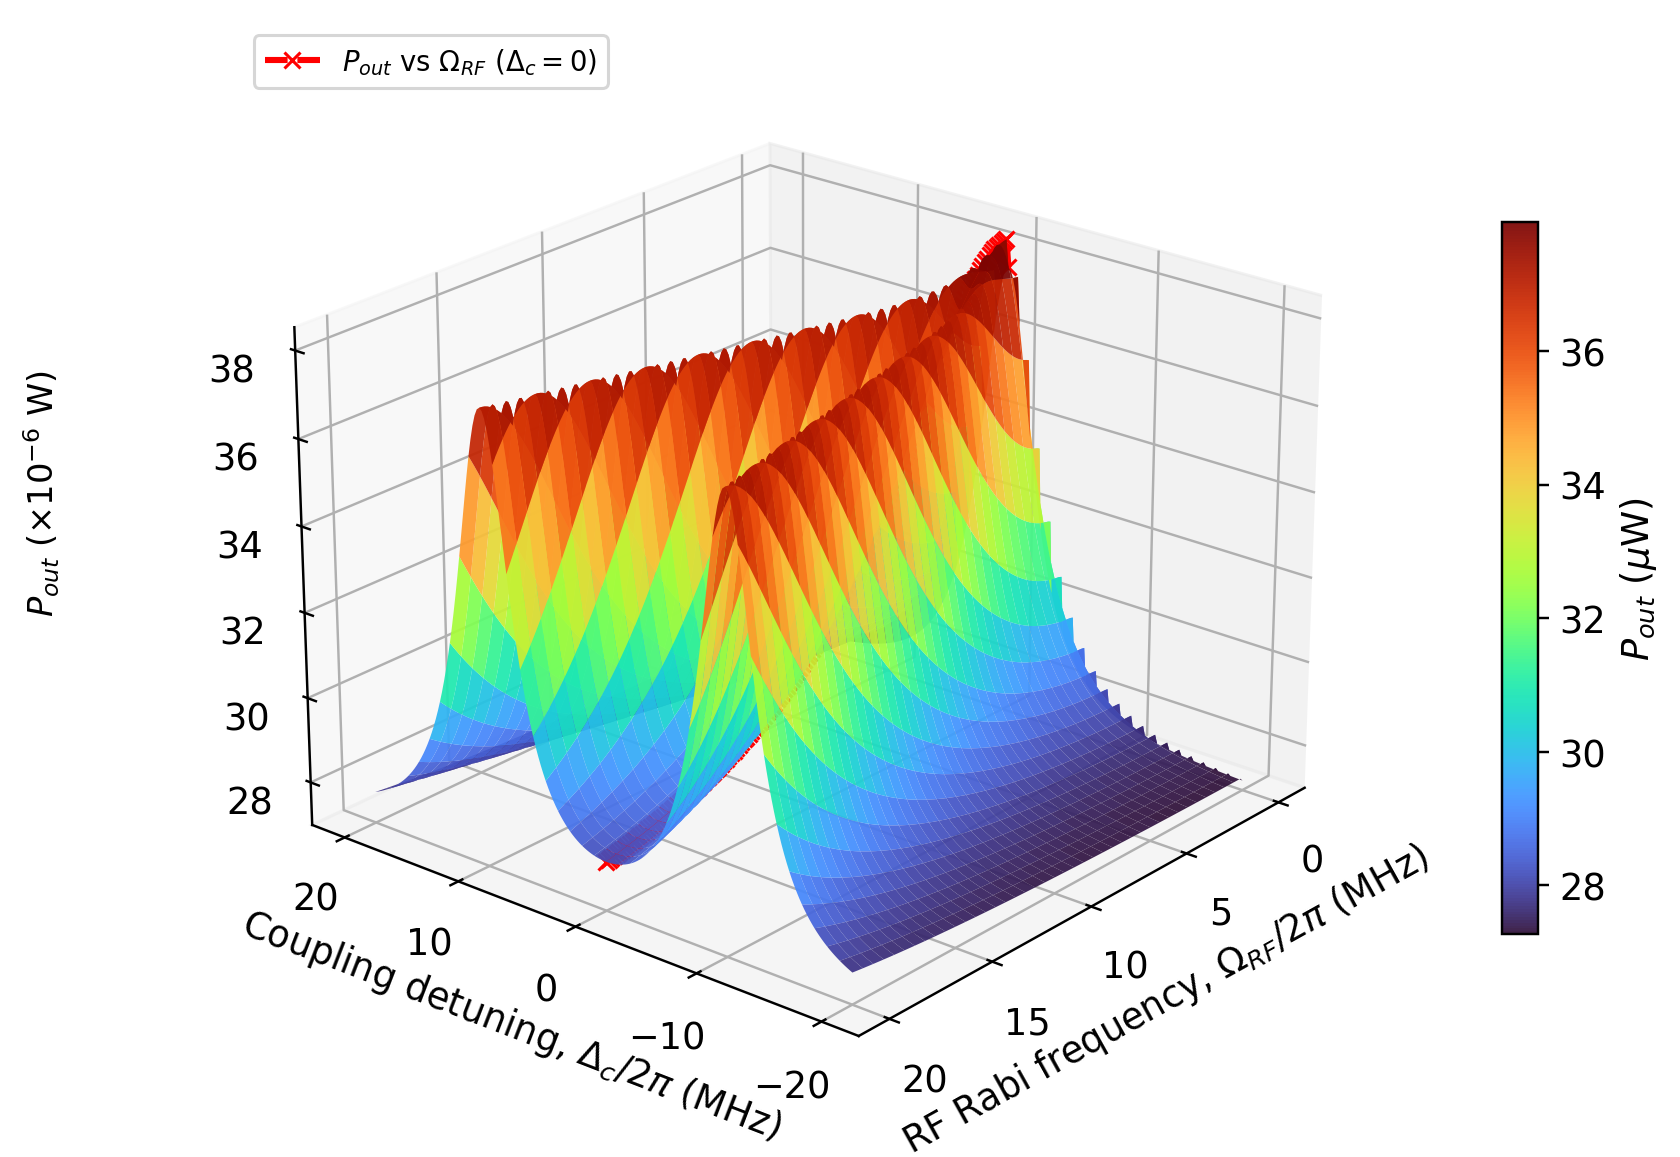
\includegraphics[width=\linewidth]{h_fig3_surface.png}
  \caption{$P_{out}$ versus $\Delta_c$ and $\Omega_{RF}$.}
\end{subfigure}\hfill
\begin{subfigure}{0.49\textwidth}
  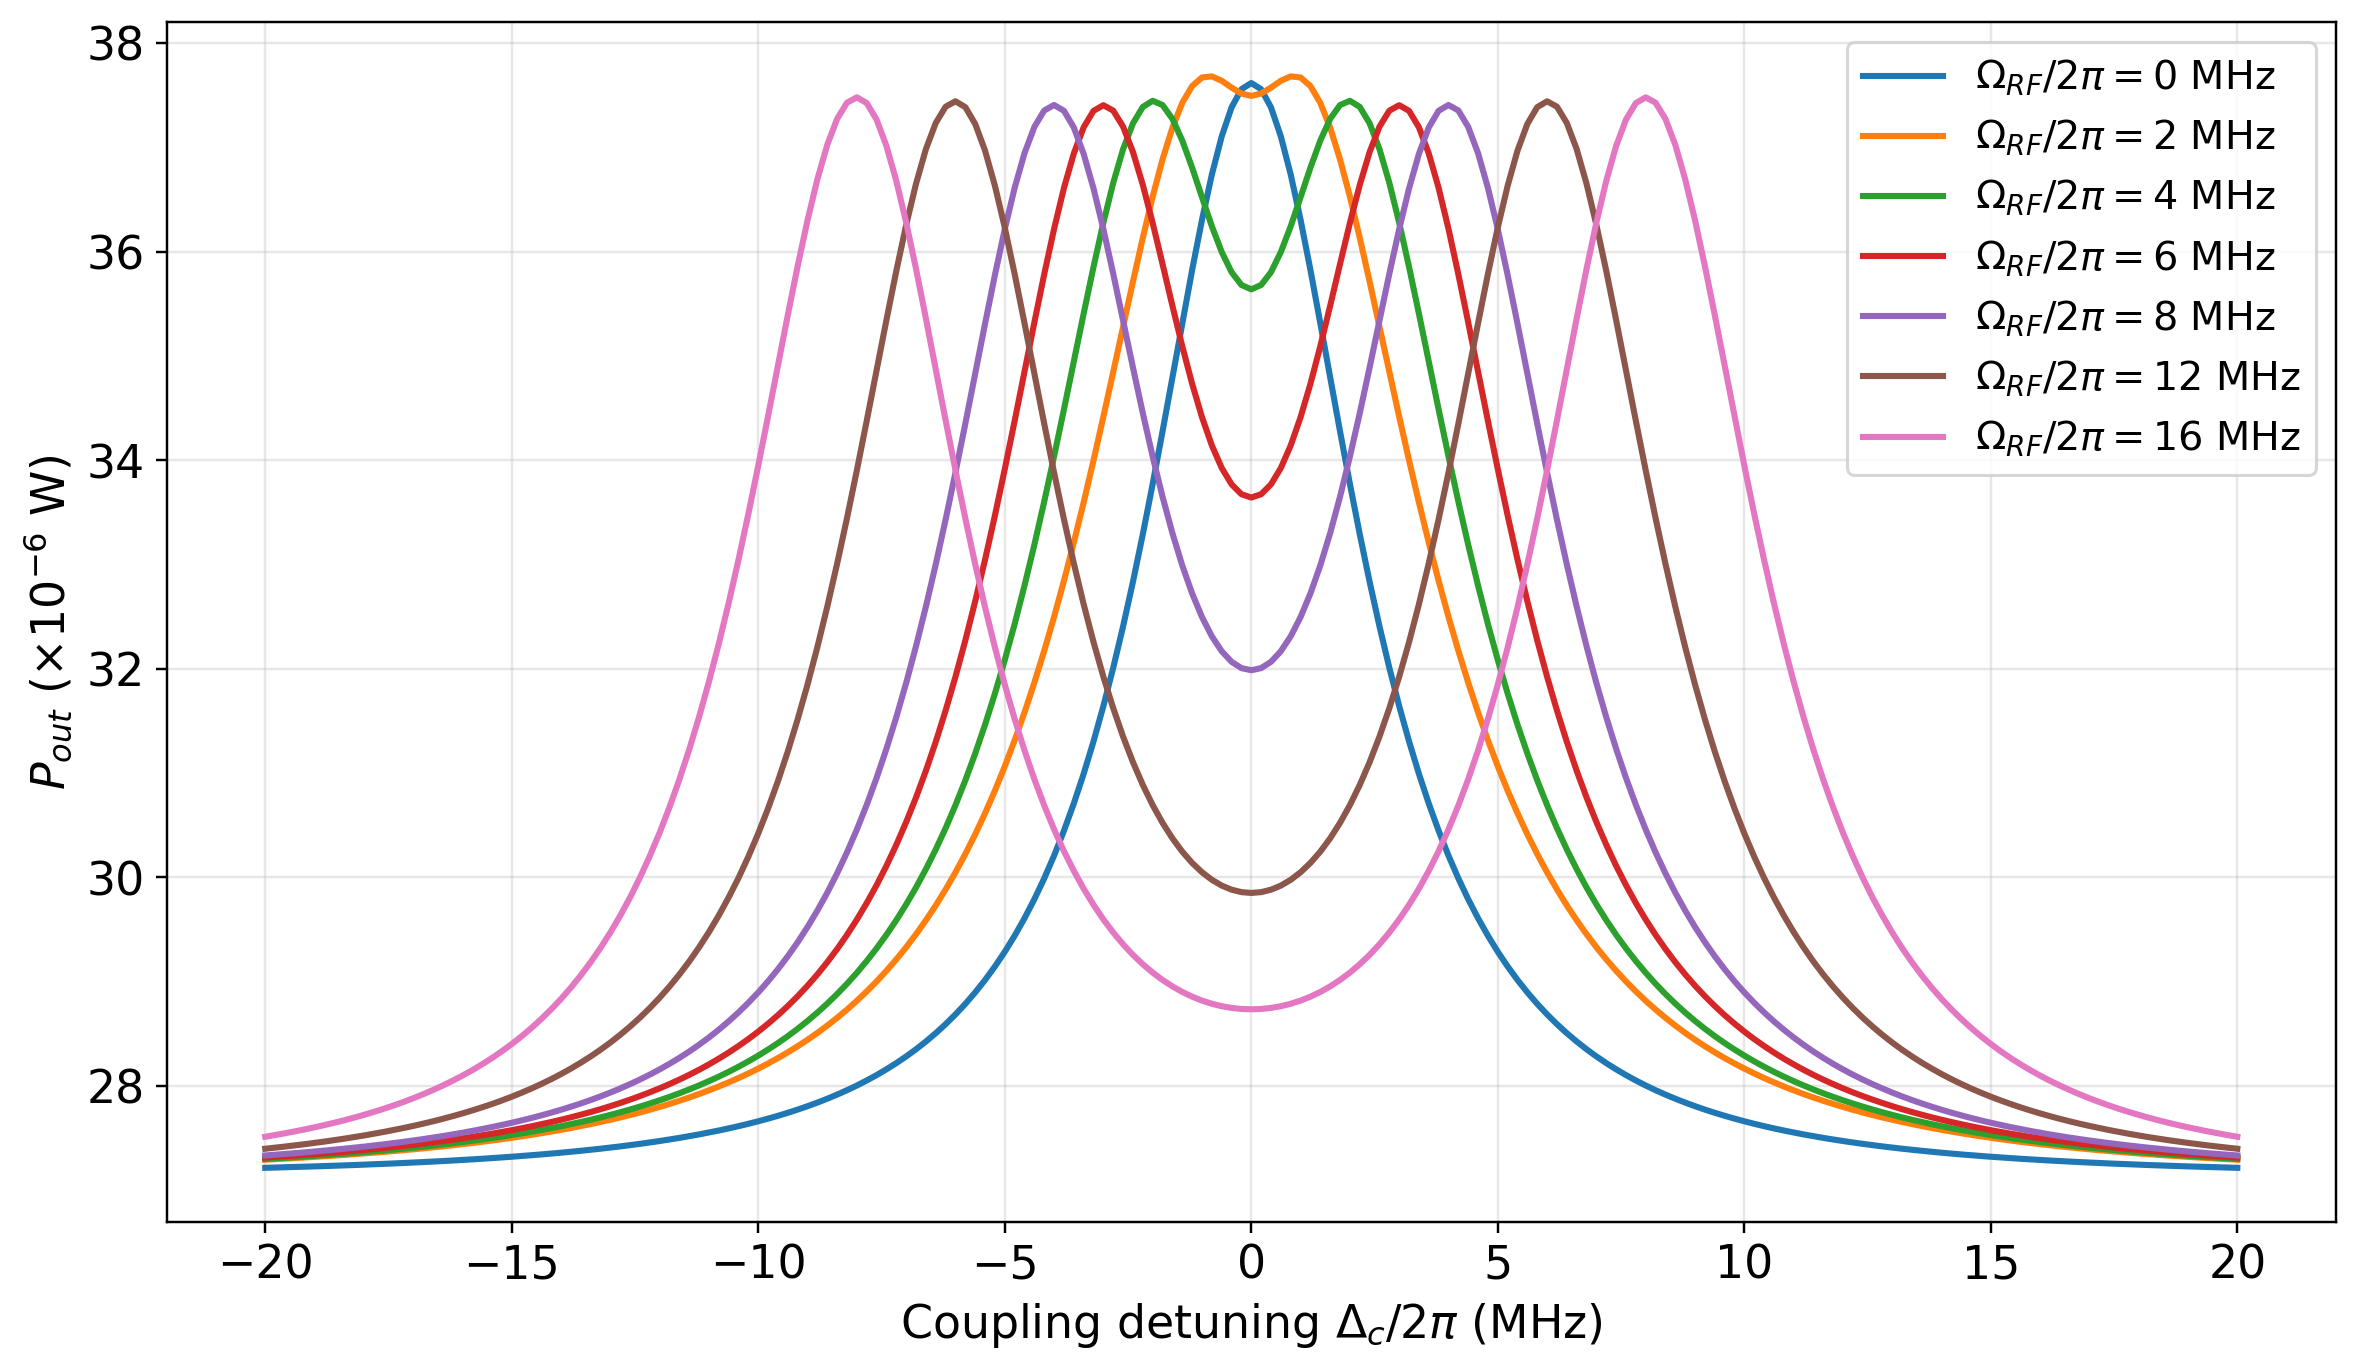
\includegraphics[width=\linewidth]{h_fig3_slices.png}
  \caption{Spectra at fixed $\Omega_{RF}$.}
\end{subfigure}
\caption{Simulated EIT/AT response of the LO-free receiver.}
\label{fig:h3}
\end{figure}

\subsection{\texorpdfstring{Distortion of the LO-free receiver (Fig.~4 of~\cite{chen2025harnessing})}{Distortion of the LO-free receiver (Fig. 4)}}

For every value of $\Omega_{RF}$ in Fig.~\ref{fig:h3}(a), the positions of the two AT peaks were
located. The splitting is considered resolvable when the distance between the peaks is larger
than the EIT linewidth, measured as $5.19$~MHz (FWHM) from the spectrum at $\Omega_{RF}=0$.
The result is shown in Fig.~\ref{fig:h4}.
\begin{itemize}[leftmargin=*,itemsep=2pt]
  \item \textit{How the graph is obtained:} Fig.~\ref{fig:h3} data (no new solution)
        $\rightarrow$ locate the two AT peaks in each row of fixed $\Omega_{RF}$ $\rightarrow$
        peak separation $\rightarrow$ compare with the EIT linewidth (FWHM at $\Omega_{RF}=0$)
        $\rightarrow$ resolvable / not resolvable $\rightarrow$ threshold $\Omega_{RF,th}$.
  \item Above the threshold the peak positions follow $\Delta_c=\pm\Omega_{RF}/2$, since the AT
        splitting is set by the RF Rabi frequency.
  \item Below $\Omega_{RF}/2\pi=5.125$~MHz the two peaks lie within the EIT linewidth and merge
        into one, so $\Omega_{RF}$ can no longer be read from the splitting. This is the
        distortion region of the LO-free receiver.
  \item The threshold depends on the resolvability criterion. With the FWHM criterion used
        here it is $5.125$~MHz, close to the value of about $5.5$~MHz in the paper.
\end{itemize}

\begin{figure}[H]
\centering
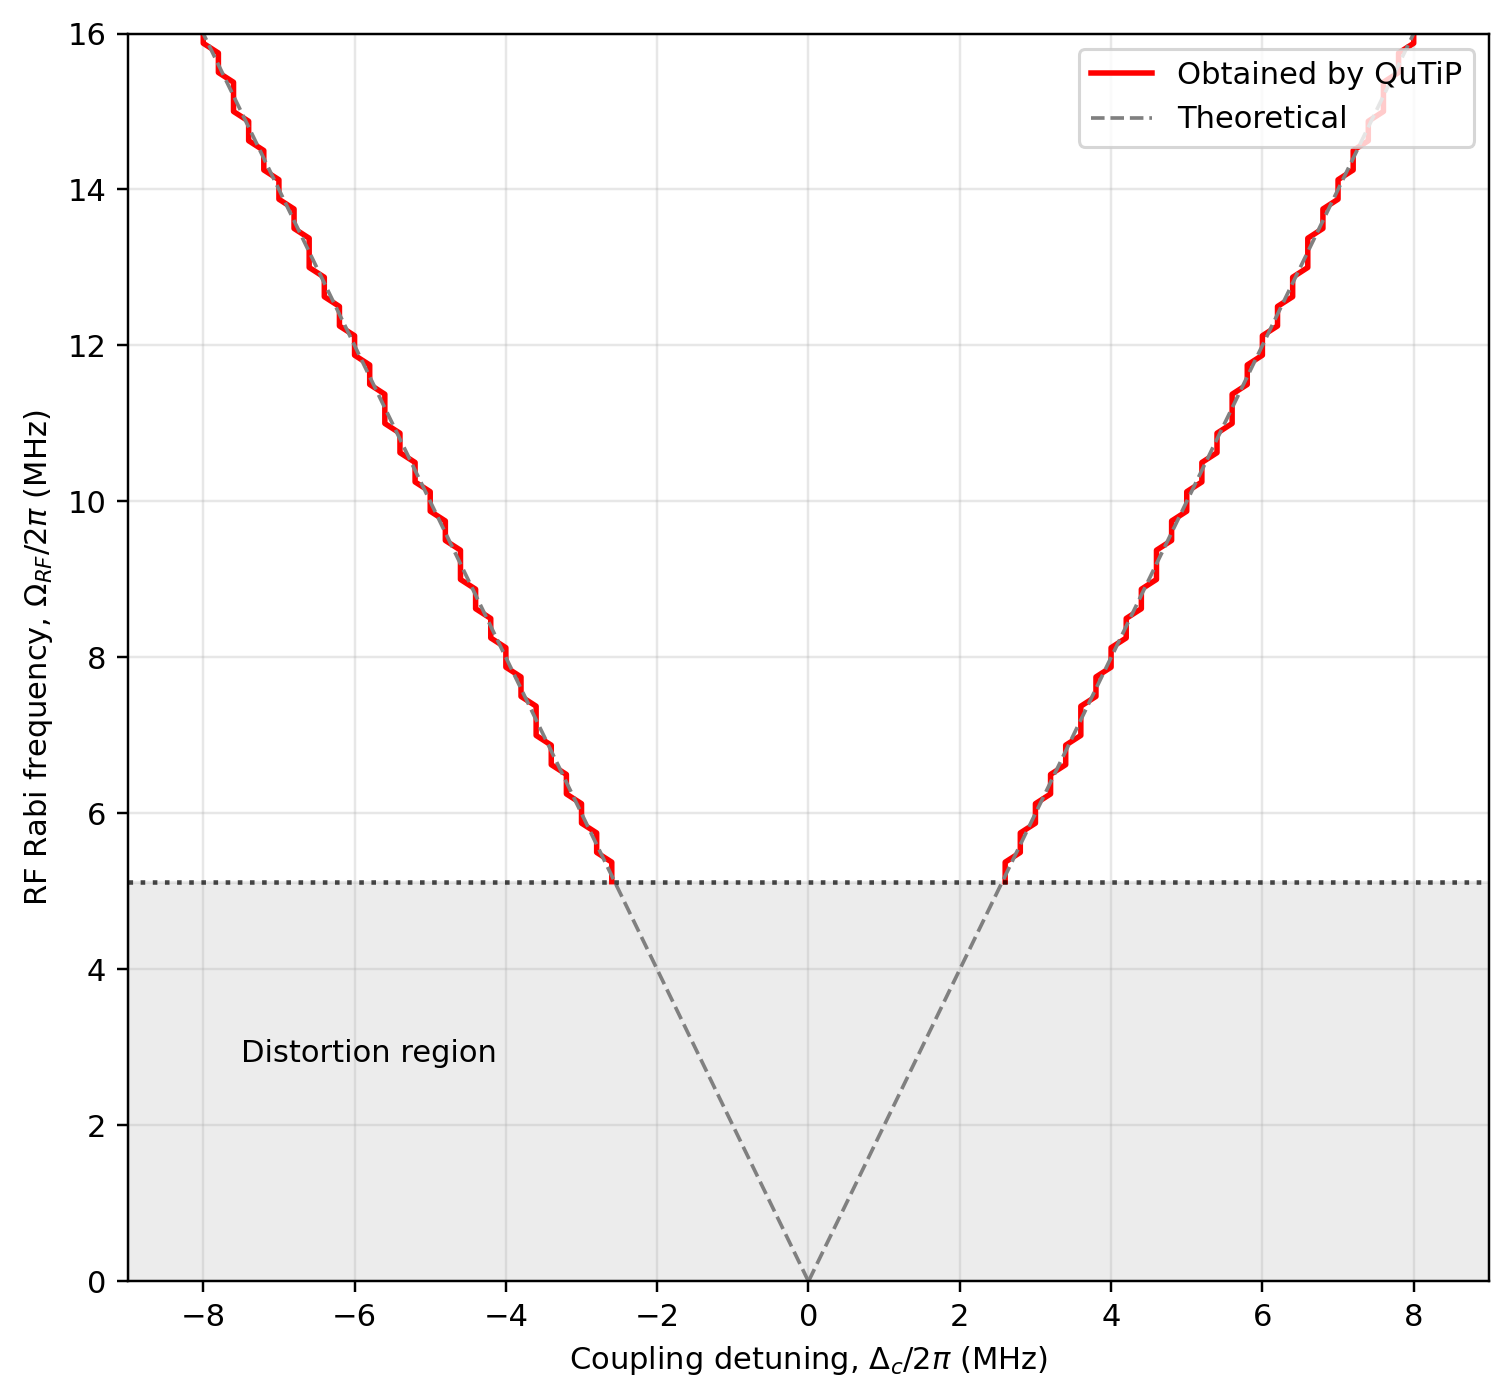
\includegraphics[width=0.55\textwidth]{h_fig4_distortion.png}
\caption{Distortion region of the LO-free receiver. Red: AT peak positions from QuTiP; dashed: $\Delta_c=\pm\Omega_{RF}/2$.}
\label{fig:h4}
\end{figure}

\subsection{\texorpdfstring{Linear dynamic range of the LO-dressed receiver (Fig.~5 of~\cite{chen2025harnessing})}{Linear dynamic range of the LO-dressed receiver (Fig. 5)}}

For the LO-dressed receiver, $\gamma_3=\gamma_4=0$ and zero detunings are used as in the paper,
and $P_{out}$ is computed against $\Omega_{total}$ using 160 QuTiP solutions
(Fig.~\ref{fig:h5}(a)). A straight line was fitted around the operating point
$\Omega_{LO}/2\pi=4.23$~MHz, and the fitting window was widened as long as $R^2\geq0.998$. This
gives a linear dynamic range of $[1.03,\,7.36]$~MHz, while the paper shows roughly
$[1.3,\,7.2]$~MHz. In Fig.~\ref{fig:h5}(b)--(c), $\Omega_{total}(t)$ is passed through this
curve.
\begin{itemize}[leftmargin=*,itemsep=2pt]
  \item \textit{How the graph is obtained:} (a) $\Omega_{total}$ grid $\rightarrow$
        Hamiltonian with $\Omega=\Omega_{total}$ $\rightarrow$ QuTiP $\rho_{21}$ $\rightarrow$
        $P_{out}(\Omega_{total})$ $\rightarrow$ straight-line fit around $\Omega_{LO}$
        $\rightarrow$ slope $\kappa$ and linear range. (b) $\Omega_{RF}$, $\Delta f$
        $\rightarrow$ $\Omega_{total}(t)=|\Omega_{LO}+e^{j2\pi\Delta f t}\Omega_{RF}|$.
        (c) $\Omega_{total}(t)$ $\rightarrow$ interpolated curve of (a) $\rightarrow$
        $P_{out}(t)$.
  \item Around $\Omega_{LO}$ the transmission changes almost linearly with $\Omega_{total}$, so
        a weak RF field gives an output proportional to $\Omega_{RF}$. This is the mixer
        behaviour described by~\eqref{eq:pout_lod}.
  \item For $\Omega_{RF}=1$ and $3$~MHz, $\Omega_{total}(t)$ stays inside the linear range and
        the output remains nearly sinusoidal.
  \item For $\Omega_{RF}=5$~MHz, $\Omega_{RF}/\Omega_{LO}=1.18$, so $\Omega_{total}(t)$ leaves
        the linear range and the output becomes clearly asymmetric (distorted).
  \item The fitted slope is $\kappa\approx-1.05~\mu$W per MHz of $\Omega_{total}/2\pi$
        ($R^2=0.998$). It is negative because a larger $\Omega_{total}$ splits the EIT peak further
        apart, so less probe light is transmitted at $\Delta_c=0$.
  \item In Fig.~\ref{fig:h5}(b), $\Omega_{total}(t)$ oscillates between
        $|\Omega_{LO}-\Omega_{RF}|$ and $\Omega_{LO}+\Omega_{RF}$ once per beat period
        $1/\Delta f=6.67~\mu$s. The operating point $\Omega_{LO}/2\pi=4.23$~MHz lies near the
        middle of the linear range, so the largest RF amplitude that is still received without
        distortion is about $3.1$~MHz on either side.
  \item The magnitude $\kappa$ sets the gain of the atomic mixer: it appears squared in the
        LO-dressed SNR~\eqref{eq:snr_lod}, so a steeper slope at the operating point directly
        gives a higher SNR.
\end{itemize}

\begin{figure}[H]
\centering
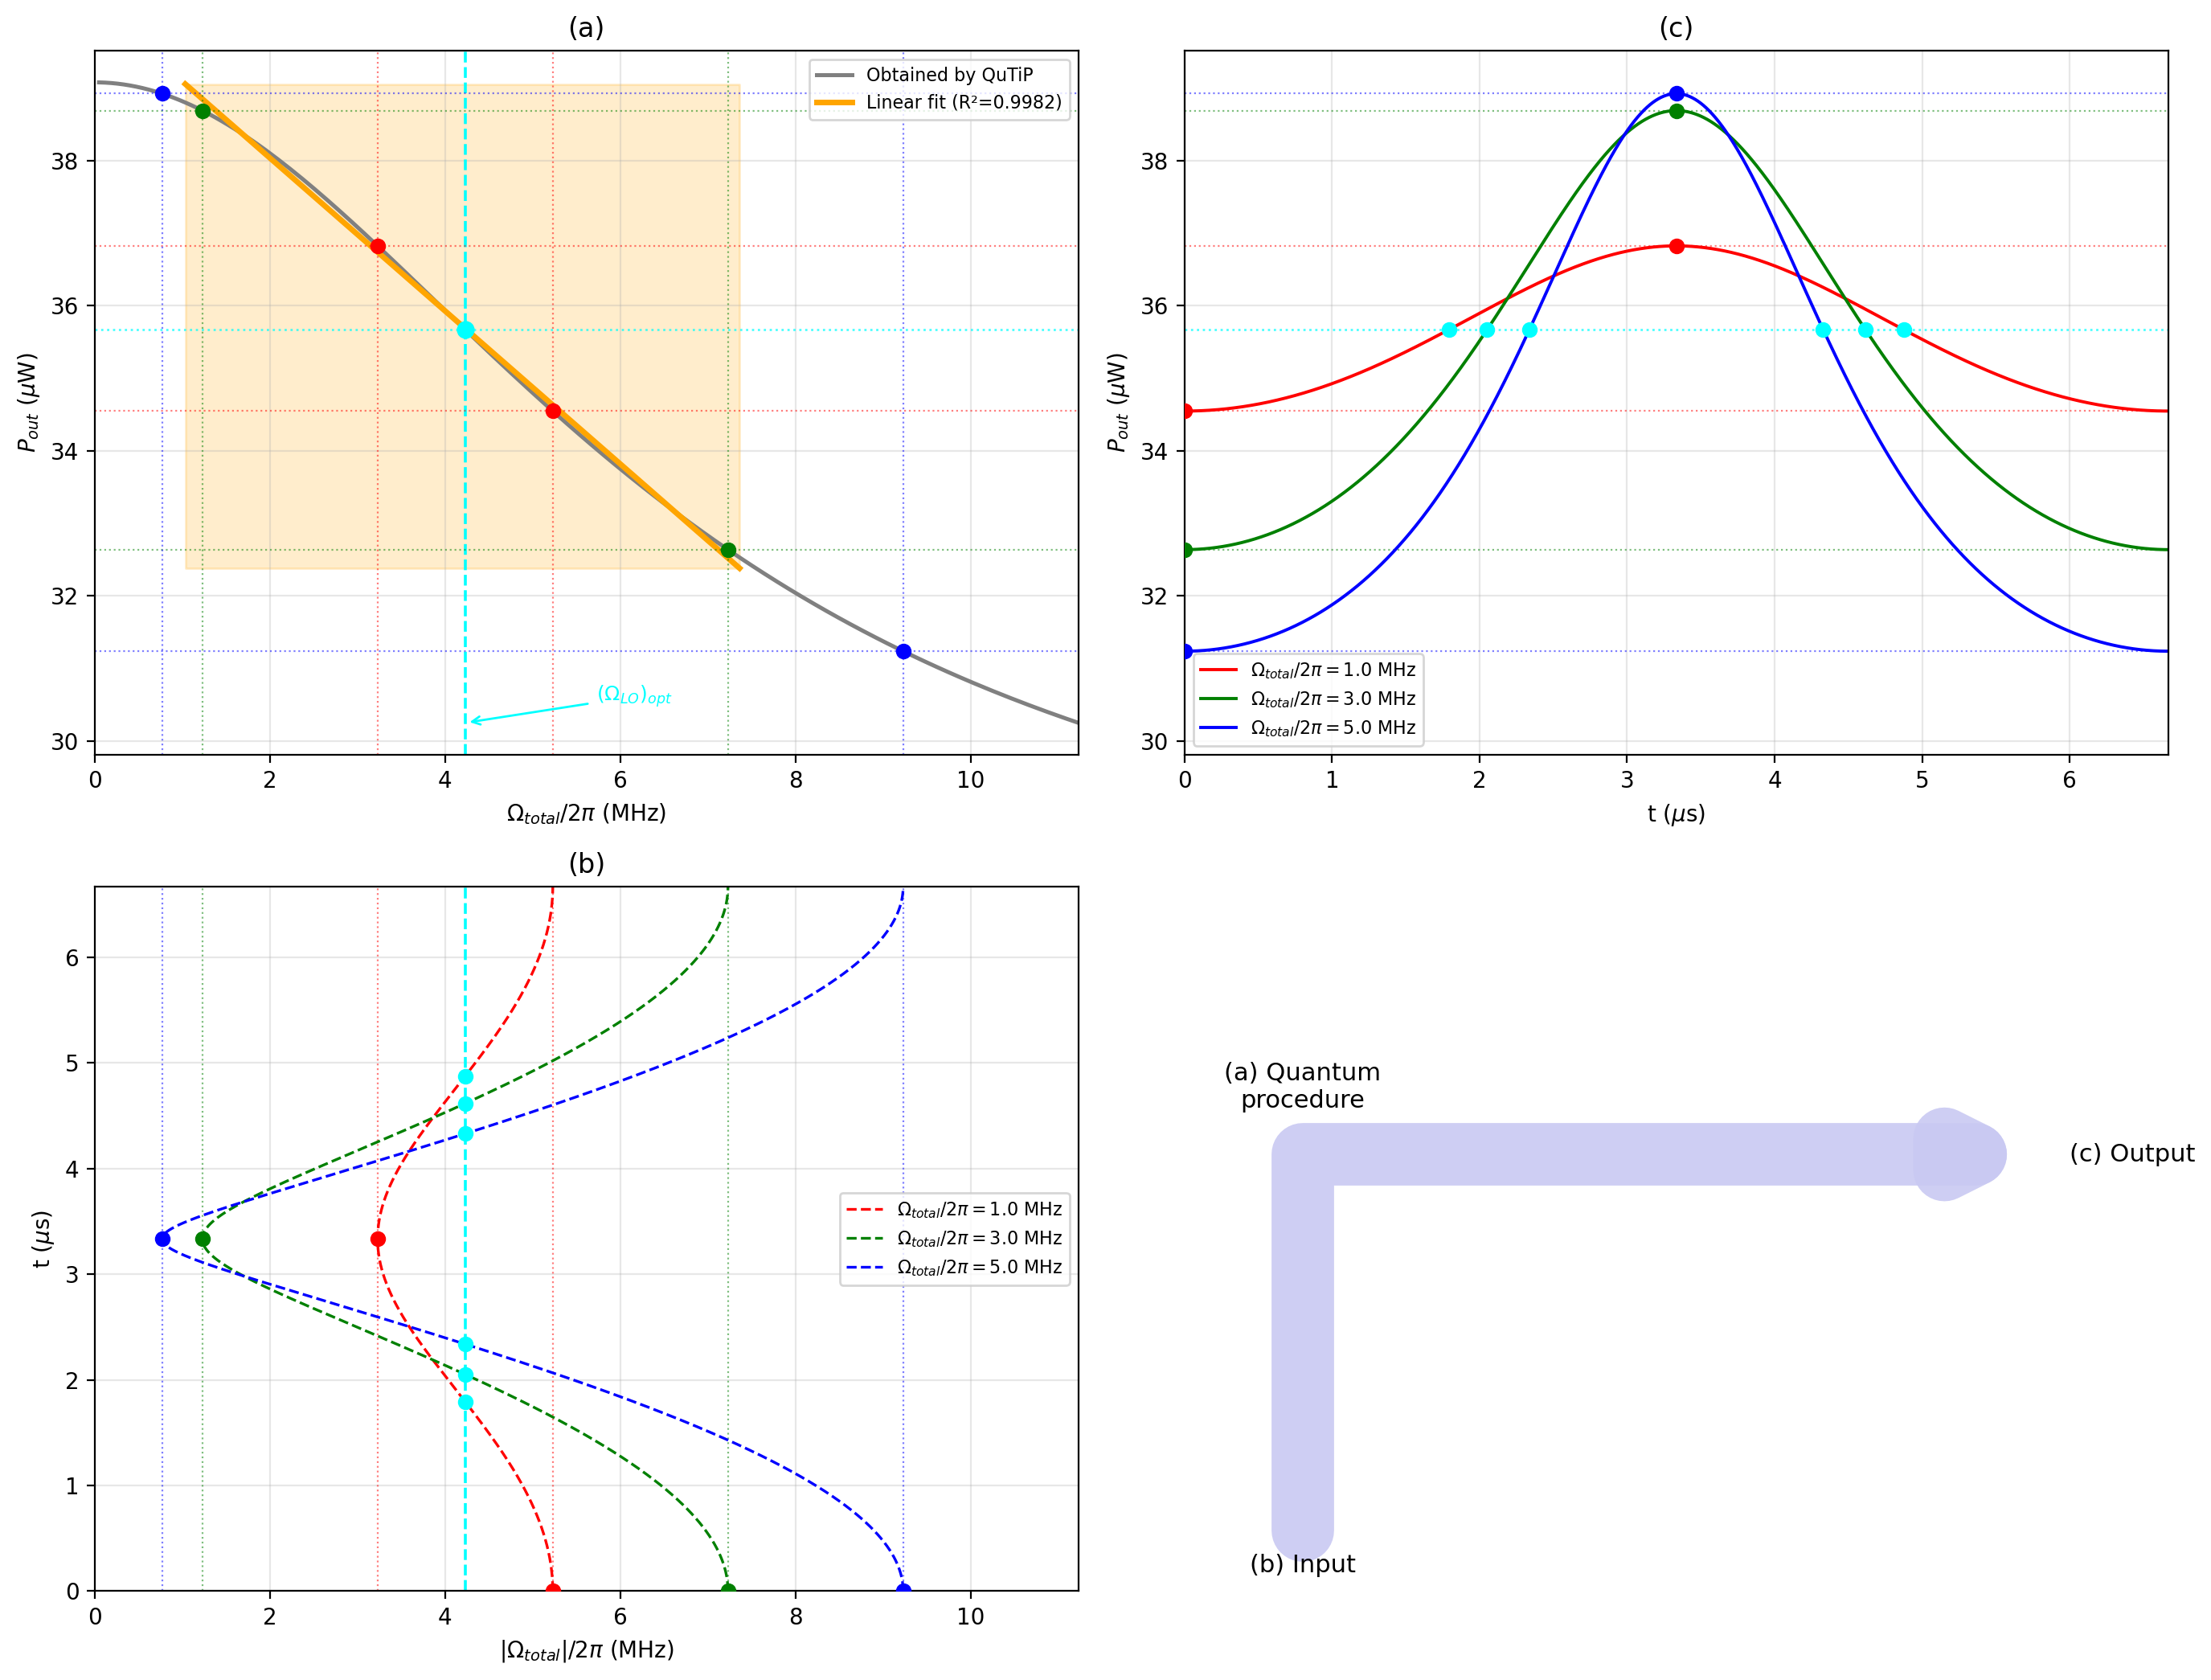
\includegraphics[width=0.85\textwidth]{h_fig5_lodressed.png}
\caption{LO-dressed receiver: (a) $P_{out}$ versus $\Omega_{total}$ with the linear fit, (b) input $\Omega_{total}(t)$, (c) output $P_{out}(t)$ over one period $1/\Delta f$.}
\label{fig:h5}
\end{figure}

\subsection{\texorpdfstring{SNR versus distance (Fig.~6 of~\cite{chen2025harnessing})}{SNR versus distance (Fig. 6)}}

Figure~\ref{fig:h6} compares the SNR of the four receivers as a function of distance, using the
link budget and \eqref{eq:snr_lofree}--\eqref{eq:snr_lod}. For the ``practical'' LO-dressed
curve, the full nonlinear QuTiP response is used instead of the linear slope $\kappa$.
\begin{itemize}[leftmargin=*,itemsep=2pt]
  \item \textit{How the graph is obtained:} distance $d$ $\rightarrow$
        $P_{Rx}=P_{Tx}G_{Tx}\eta_0/(4\pi d^2)$ $\rightarrow$ $\Omega_{RF}\propto\sqrt{P_{Rx}}$.
        Conventional: power collected by an aperture $\lambda_{RF}^2/4\pi$ $\rightarrow$ SNR
        with background and thermal noise. LO-free: $P_{Rx}$ $\rightarrow$~\eqref{eq:snr_lofree},
        plotted only where $\Omega_{RF}\geq\Omega_{RF,th}$ (Fig.~\ref{fig:h4}). Theoretical
        LO-dressed: $\kappa$ from Fig.~\ref{fig:h5} $\rightarrow$~\eqref{eq:snr_lod}. Practical
        LO-dressed: $\Omega_{RF}$ $\rightarrow$ $\Omega_{total}(t)$ $\rightarrow$ $P_{out}(t)$
        from a wider QuTiP sweep of $P_{out}(\Omega_{total})$ (up to 35~MHz) $\rightarrow$
        Fourier amplitude $|P(\Delta f)|$ $\rightarrow$ SNR with the same noise.
  \item The LO-free SNR saturates at $1/\tilde\epsilon^2=46.02$~dB, because the observation
        uncertainty in~\eqref{eq:snr_lofree} grows with the field. The curve ends after a few
        metres, where the receiver enters its distortion region.
  \item The practical LO-dressed receiver is worse than the theoretical one at short distances,
        where the strong RF field pushes $\Omega_{total}$ outside the linear range.
  \item At larger distances the LO-dressed SNR decreases at the same rate as that of the
        conventional receiver, since both are proportional to $P_{Rx}$. Its advantage is
        therefore a constant gain, $28.9$~dB at 100~m for $P_{Tx}=-10$~dBm, compared with
        about 44~dB reported in the paper.
\end{itemize}

\begin{figure}[H]
\centering
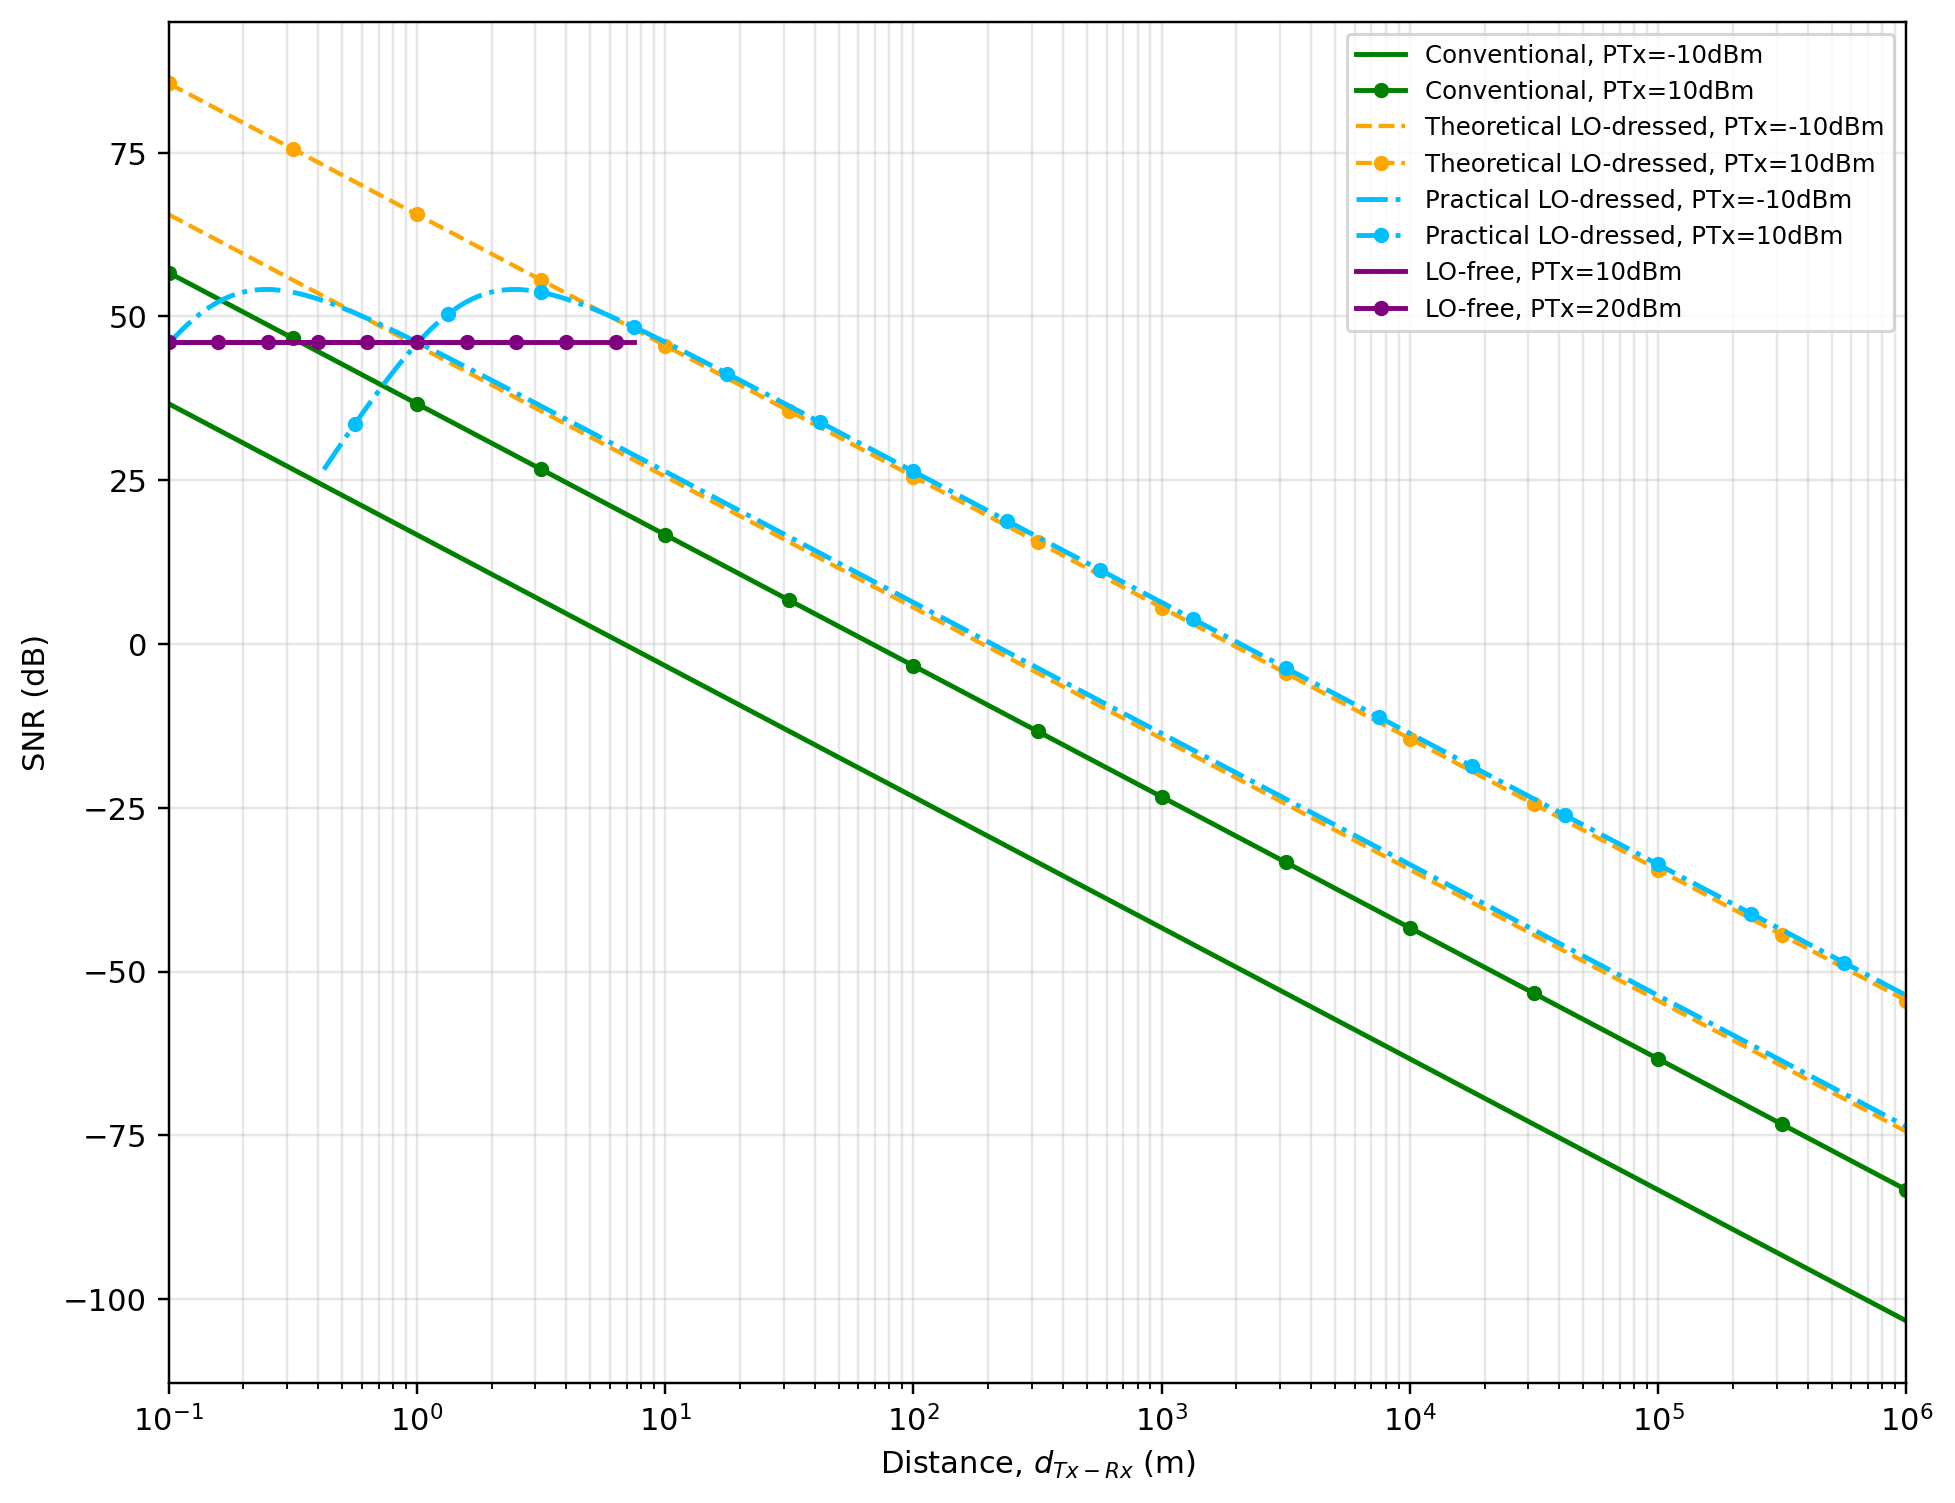
\includegraphics[width=0.62\textwidth]{h_fig6_snr_distance.png}
\caption{SNR versus distance for the conventional, LO-free, theoretical LO-dressed and practical LO-dressed receivers.}
\label{fig:h6}
\end{figure}

\subsection{Comparison with the paper}

Table~\ref{tab:hcompare} compares the main simulated values with those reported in the paper.

\begin{table}[H]
\centering
\caption{Values reported in~\cite{chen2025harnessing} and simulated values.}
\label{tab:hcompare}
\small
\renewcommand{\arraystretch}{1.15}
\begin{tabular}{lll}
\toprule
\textbf{Quantity} & \textbf{Paper} & \textbf{Simulated}\\
\midrule
AT peak positions & $\Delta_c=\pm\Omega_{RF}/2$ & same\\
LO-free distortion threshold & about $5.5$~MHz & $5.125$~MHz\\
LO-dressed linear dynamic range & about $[1.3,7.2]$~MHz & $[1.03,7.36]$~MHz\\
Peak $P_{out}$ of the EIT spectrum & about $9.6~\mu$W & $38.3~\mu$W ($P_{in}=39.1~\mu$W from Eq.~3)\\
LO-dressed SNR gain at 100~m & about $44$~dB & $28.9$~dB\\
LO-free SNR limit & not mentioned & $1/\tilde\epsilon^2=46.02$~dB\\
\bottomrule
\end{tabular}
\end{table}

% =========================================================
% 5. IMPLEMENTATION II
% =========================================================

\section{Simulation of Channel Estimation (Xu \textit{et al.})}
\label{sec:impl2}

\subsection{Algorithms}

Three estimators are implemented. Biased GS works on the exact magnitude model and is used as
the 1D baseline; GD and PGD work on the linearised model~\eqref{eq:lin}. In all of them
$\mathbf S\in\mathbb C^{K\times P}$ holds the pilots, and the iterations stop when the change
$\|\mathbf G^{t+1}-\mathbf G^{t}\|_F^2$ falls below $\epsilon$ or after $T_{\max}$ iterations.

\begin{itemize}[leftmargin=*,itemsep=2pt]
  \item \textit{Notation.} $\mathbf Y\in\mathbb R^{I\times P}$ holds the measured magnitudes
        $y_{i,p}$, $\mathbf B\in\mathbb C^{I\times P}$ the known reference, $\mathbf Z$ its phase
        terms $Z_{i,p}=e^{-j\angle b_{i,p}}$, and $\mathbf G\in\mathbb C^{I\times K}$ the unknown
        channel, with one row per vapour cell and one column per user.
  \item \textit{Biased GS} (Algorithm~\ref{alg:gs}) does not use the Taylor approximation. It
        alternates between estimating the unknown phase of each measurement and solving a
        linear least-squares problem for the channel. A spectral initialisation is needed
        because the problem is non-convex and a random start can converge to a poor solution.
  \item \textit{GD} (Algorithm~\ref{alg:gd}) minimises the least-squares cost of the linearised
        model, which is quadratic in $\mathbf G$. It starts from a random
        $\mathbf G^0\sim\mathcal{CN}(0,0.1)$, as in~\cite{xu2025channel}, and a simple step-size
        halving keeps every iteration decreasing the cost. Its complexity per iteration is
        $\mathcal O(PKI)$.
  \item \textit{PGD} (Algorithm~\ref{alg:pgd}) takes the same gradient step for the 2D array and
        then projects each user's channel onto the set of rank-$L_k$ matrices. This uses the
        structure of the channel that GD ignores, which matters most when the number of pilots
        is small.
\end{itemize}

\begin{algorithm}[H]
\caption{Biased Gerchberg--Saxton (GS), 1D array~\cite{cui2025towards,netrapalli2015}}
\label{alg:gs}
\begin{algorithmic}[1]
\Require $\mathbf Y$, $\mathbf S$, $\mathbf B$, $T_{\max}$, $\epsilon$
\State \textbf{Spectral initialisation:}
\For{$i=1,\dots,I$}
  \State $\bar{\mathbf A}_i=[\mathbf S^T\;\;\mathbf b_i]$,\quad
         $\mathbf M_i=\sum_{p=1}^{P}y_{i,p}\,\bar{\mathbf a}_{i,p}\bar{\mathbf a}_{i,p}^H$
         \Comment{$\bar{\mathbf a}_{i,p}$: $p$th row of $\bar{\mathbf A}_i$}
  \State $\mathbf v_i\gets$ principal eigenvector of $\mathbf M_i$
  \State $r_i=|\bar{\mathbf A}_i\mathbf v_i|^T\mathbf y_i/\|\bar{\mathbf A}_i\mathbf v_i\|_2^2$,\quad
         $\bar{\mathbf g}_i=r_i\mathbf v_i$
  \State $\bar{\mathbf g}_i\gets e^{-j\angle[\bar{\mathbf g}_i]_{K+1}}\,\bar{\mathbf g}_i$,\quad
         $\mathbf g_i^{(0)}=[\bar{\mathbf g}_i]_{1:K}$
         \Comment{remove the reference phase}
\EndFor
\State $\mathbf G^{(0)}=[\mathbf g_1^{(0)},\dots,\mathbf g_I^{(0)}]^T$
\State \textbf{GS iterations:}
\For{$t=1,\dots,T_{\max}$}
  \State $\mathbf X^{(t)}=\mathbf G^{(t-1)}\mathbf S+\mathbf B$,\quad
         $\bm\Theta^{(t)}=\angle\mathbf X^{(t)}$
         \Comment{phase estimate}
  \State $\mathbf R^{(t)}=\mathbf Y\circ e^{j\bm\Theta^{(t)}}$
  \State $\mathbf G^{(t)}=(\mathbf R^{(t)}-\mathbf B)\,\mathbf S^H(\mathbf S\mathbf S^H)^{-1}$
         \Comment{least-squares update}
  \If{$\|\mathbf G^{(t)}-\mathbf G^{(t-1)}\|_F^2\leq\epsilon$} \textbf{break}
  \EndIf
\EndFor
\State \Return $\hat{\mathbf G}=\mathbf G^{(t)}$
\end{algorithmic}
\end{algorithm}

\begin{algorithm}[H]
\caption{Gradient descent (GD), 1D array~\cite{xu2025channel}}
\label{alg:gd}
\begin{algorithmic}[1]
\Require $\mathbf Y$, $\mathbf S$, $\mathbf Z$, $\mathbf B$, $\mathbf G^0$, $T_{\max}$, $\epsilon$
\State $t=0$
\Repeat
  \State $\hat{\mathbf Y}^t=\mathrm{Re}\{\mathbf Z\circ(\mathbf G^t\mathbf S)\}+|\mathbf B|$
         \Comment{linearised prediction}
  \State $\mathbf E^t=\mathbf Y-\hat{\mathbf Y}^t$
  \State $\mathbf D^t=-2\,(\mathbf E^t\circ\mathbf Z^*)\,\mathbf S^H$
         \Comment{gradient of $\mathcal L(\mathbf G)=\|\mathbf E\|_F^2$}
  \State $\eta_t=1$; halve $\eta_t$ until $\mathcal L(\mathbf G^t-\eta_t\mathbf D^t)<\mathcal L(\mathbf G^t)$
  \State $\mathbf G^{t+1}=\mathbf G^t-\eta_t\mathbf D^t$,\quad $t\gets t+1$
\Until{$\|\mathbf G^{t}-\mathbf G^{t-1}\|_F^2<\epsilon$ \textbf{or} $t\geq T_{\max}$}
\State \Return $\hat{\mathbf G}=\mathbf G^t$
\end{algorithmic}
\end{algorithm}

\begin{algorithm}[H]
\caption{Projected gradient descent (PGD), 2D array~\cite{xu2025channel}}
\label{alg:pgd}
\begin{algorithmic}[1]
\Require Mode-3 unfolded $\mathbf Y_{(3)}$, $\mathbf Z_{(3)}$, $\mathbf B_{(3)}$; ranks $\{L_k\}$; $\mathbf S$; $T_{\max}$, $\epsilon$
\State Initialise $\mathbf G_{(3)}^0\in\mathbb C^{K\times I_1I_2}$, $t=0$
\Repeat
  \State $\nabla f=-\mathbf S^*\big[(\mathbf Y_{(3)}-|\mathbf B_{(3)}|-\mathrm{Re}\{\mathbf Z_{(3)}\circ(\mathbf S^T\mathbf G^t_{(3)})\})\circ\mathbf Z^*_{(3)}\big]$
  \State $\mathbf M=\mathbf G^t_{(3)}-\zeta^t\,\nabla f$
         \Comment{gradient step}
  \For{$k=1,\dots,K$}
    \State $\mathbf U_k\bm\Sigma_k\mathbf V_k^H=\mathrm{svd}\big(\mathrm{mat}([\mathbf M]_{k,:})\big)$
           \Comment{$I_1\times I_2$ matrix}
    \State $[\mathbf X]_{k,:}=\mathrm{vec}\big(\tilde{\mathbf U}_k\tilde{\bm\Sigma}_k\tilde{\mathbf V}_k^H\big)^T$
           \Comment{keep the $L_k$ largest singular values}
  \EndFor
  \State $\mathbf G^{t+1}_{(3)}=\mathbf X$,\quad $t\gets t+1$
\Until{$\|\mathbf G^{t}_{(3)}-\mathbf G^{t-1}_{(3)}\|_F^2<\epsilon$ \textbf{or} $t\geq T_{\max}$}
\State \Return $\hat{\mathbf G}_{(3)}=\mathbf G^t_{(3)}$
\end{algorithmic}
\end{algorithm}

\begin{itemize}[leftmargin=*,itemsep=2pt]
  \item Steps 6--7 of Algorithm~\ref{alg:pgd} give the best rank-$L_k$ approximation
        (Eckart--Young--Mirsky theorem). The rank is limited to $L_k$ because each propagation
        path contributes an outer product $e^{-j(i_1-1)u}e^{-j(i_2-1)v}$, which has rank one.
  \item \textit{CRLB.} For the linearised model,
        $\mathrm{CRB}(\mathbf g)=4\sigma^2[\mathbf I_{I_1I_2}\otimes(\mathbf S^*\mathbf S^T)^{-1}]$. It
        does not depend on the number of antennas and decreases with SNR and with pilot length.
\end{itemize}

\subsection{Simulation setup}

The parameters are taken from Section~V of~\cite{xu2025channel}: Rydberg levels
$52D_{5/2}\rightarrow53P_{3/2}$ ($\omega_{eg}\approx2\pi\times5$~GHz),
$\boldsymbol\mu_{eg}=[0,\,1785.9\,qa_0,\,0]^T$, $K=3$ users, $L_k$ uniform in $\{3,\dots,7\}$,
polarisation components from $\mathcal N(0,1/3)$, $\alpha_{l,k}\sim\mathcal{CN}(0,1)$,
$\alpha_b\sim\mathcal{CN}(0,10)$, pilots from $\mathcal{CN}(0,1)$, initial estimate from
$\mathcal{CN}(0,0.1)$, $I=8$ cells for 1D and $8\times8$ cells for 2D. Some values are not given
in the paper and were chosen as follows: half-wavelength spacing, arrival angles uniform in
$[0,2\pi)$, $\mathrm{SNR}=\mathbb E|a|^2/\sigma^2$, and in the 2D case the polarisation is drawn
once per path so that each user's channel keeps its rank-$L_k$ structure. Since the paper does not
state how the channel is normalised, only the trends and the gap from the CRLB are compared. The NMSE is computed as
$\sum\|\mathbf G-\hat{\mathbf G}\|_F^2/\sum\|\mathbf G\|_F^2$, averaged over 500 (1D), 100 (2D, SNR
sweep) and 2000 (pilot sweep) Monte Carlo runs. GD is run for at most 500 iterations, PGD for at
most 300 and GS for 100, and the iterations stop when the relative change is below $10^{-8}$.

\subsection{The strong-reference condition}

In the first set of simulations, all parameters were used exactly as given in the paper. The NMSE of
all the estimators stopped improving at around $0$~dB, far above the CRLB. To understand this,
the ratio of reference power to signal power was measured, giving
$\mathbb E|b|^2/\mathbb E|a+n|^2\approx-2$~dB. With $\alpha_b\sim\mathcal{CN}(0,10)$ and three users
having 3 to 7 paths each, the reference is actually weaker than the signal. The Taylor
approximation~\eqref{eq:lin} is then not valid, and the linearised estimator cannot reach the
CRLB. Since the paper's derivation assumes $|b|\gg|a+n|$, this condition is enforced in the
simulations shown below. The reference is kept the same in all pilot slots, as
in~\cite{cui2025towards}, and it is scaled so that $\mathbb E|b|^2/\mathbb E|a|^2=34$~dB. All other
parameters are as listed above.

\subsection{Results}

\noindent\textit{1D array.} Figure~\ref{fig:ce3} shows the NMSE of biased GS and GD together
with the CRLB.
\begin{itemize}[leftmargin=*,itemsep=2pt]
  \item More pilots give more measurements for the same unknowns, so the $P=30$ curves stay
        close to the CRLB at low and medium SNR (at 5~dB: GS $-10.5$~dB, GD $-10.2$~dB, CRLB
        $-11.6$~dB), while for $P=10$ both methods are about 4~dB above the bound.
  \item GD flattens at high SNR (about $-18.7$~dB for $P=30$) because it uses the linearised
        model: once the noise is small, the second-order term dropped in the Taylor expansion
        dominates the error. In a separate test at 30~dB SNR and $P=30$, increasing the
        reference amplitude ratio from 50 to 200 lowered the GD error from $-23.5$~dB to
        $-34.2$~dB, while ten times more iterations had no effect.
  \item GS works on the exact magnitude model, so it continues to improve and flattens at a
        lower level ($-24.7$~dB for $P=30$). For this reason, curves for different pilot lengths
        can meet at high SNR, e.g.\ GS with $P=10$ reaches the level of GD with $P=30$ at 30~dB.
\end{itemize}

\begin{figure}[H]
\centering
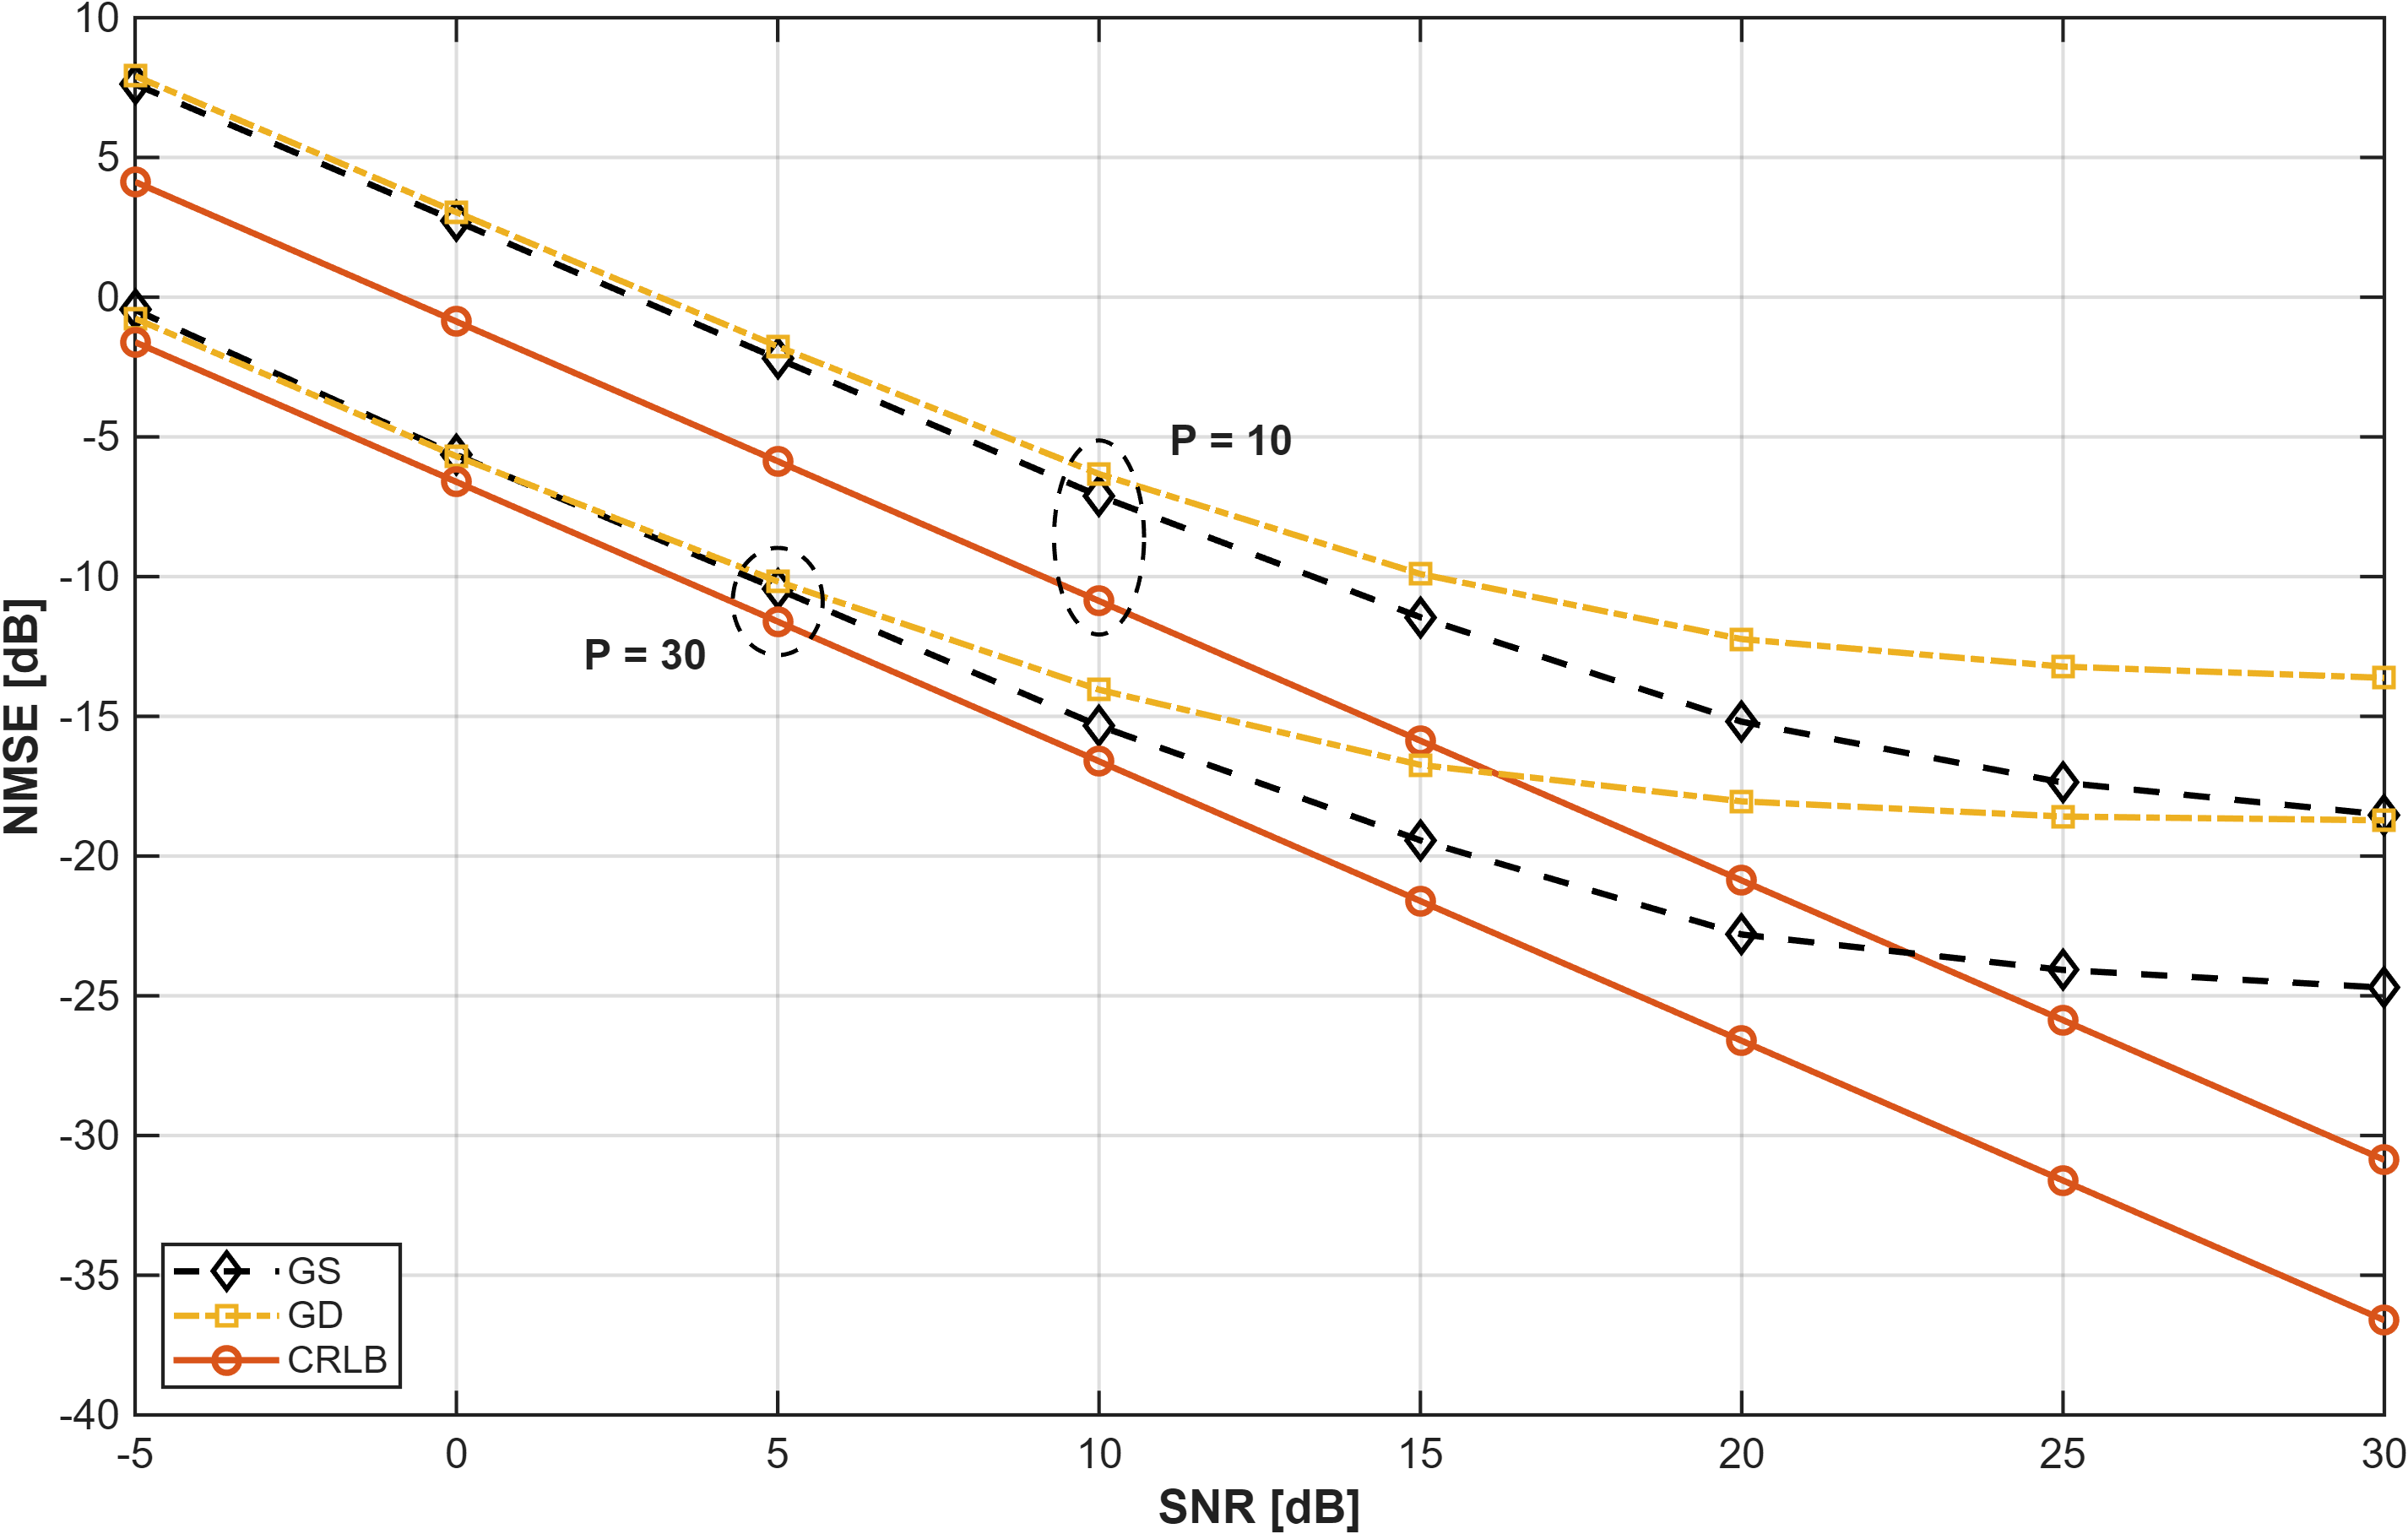
\includegraphics[width=0.75\textwidth]{ce_fig3_1d.png}
\caption{NMSE versus SNR for the 1D array ($I=8$, $K=3$, $P=10$ and $30$): biased GS, GD and CRLB.}
\label{fig:ce3}
\end{figure}

\noindent\textit{2D array.} Figure~\ref{fig:ce4} shows the results for the $8\times8$ array.
\begin{itemize}[leftmargin=*,itemsep=2pt]
  \item For $P=10$, PGD is 0.6--0.8~dB better than GD up to 15~dB SNR, because the truncated SVD
        removes the part of the estimate that does not fit the rank-$L_k$ structure.
  \item For $P=30$ the pilots alone already determine the channel well, so the projection adds
        little: the two curves nearly coincide and are within 1.3~dB of the CRLB up to 5~dB SNR,
        as in~\cite{xu2025channel}.
  \item Both methods use the linearised model, so both flatten at high SNR (about $-18$~dB for
        $P=30$), for the same reason as GD in the 1D case.
\end{itemize}

\begin{figure}[H]
\centering
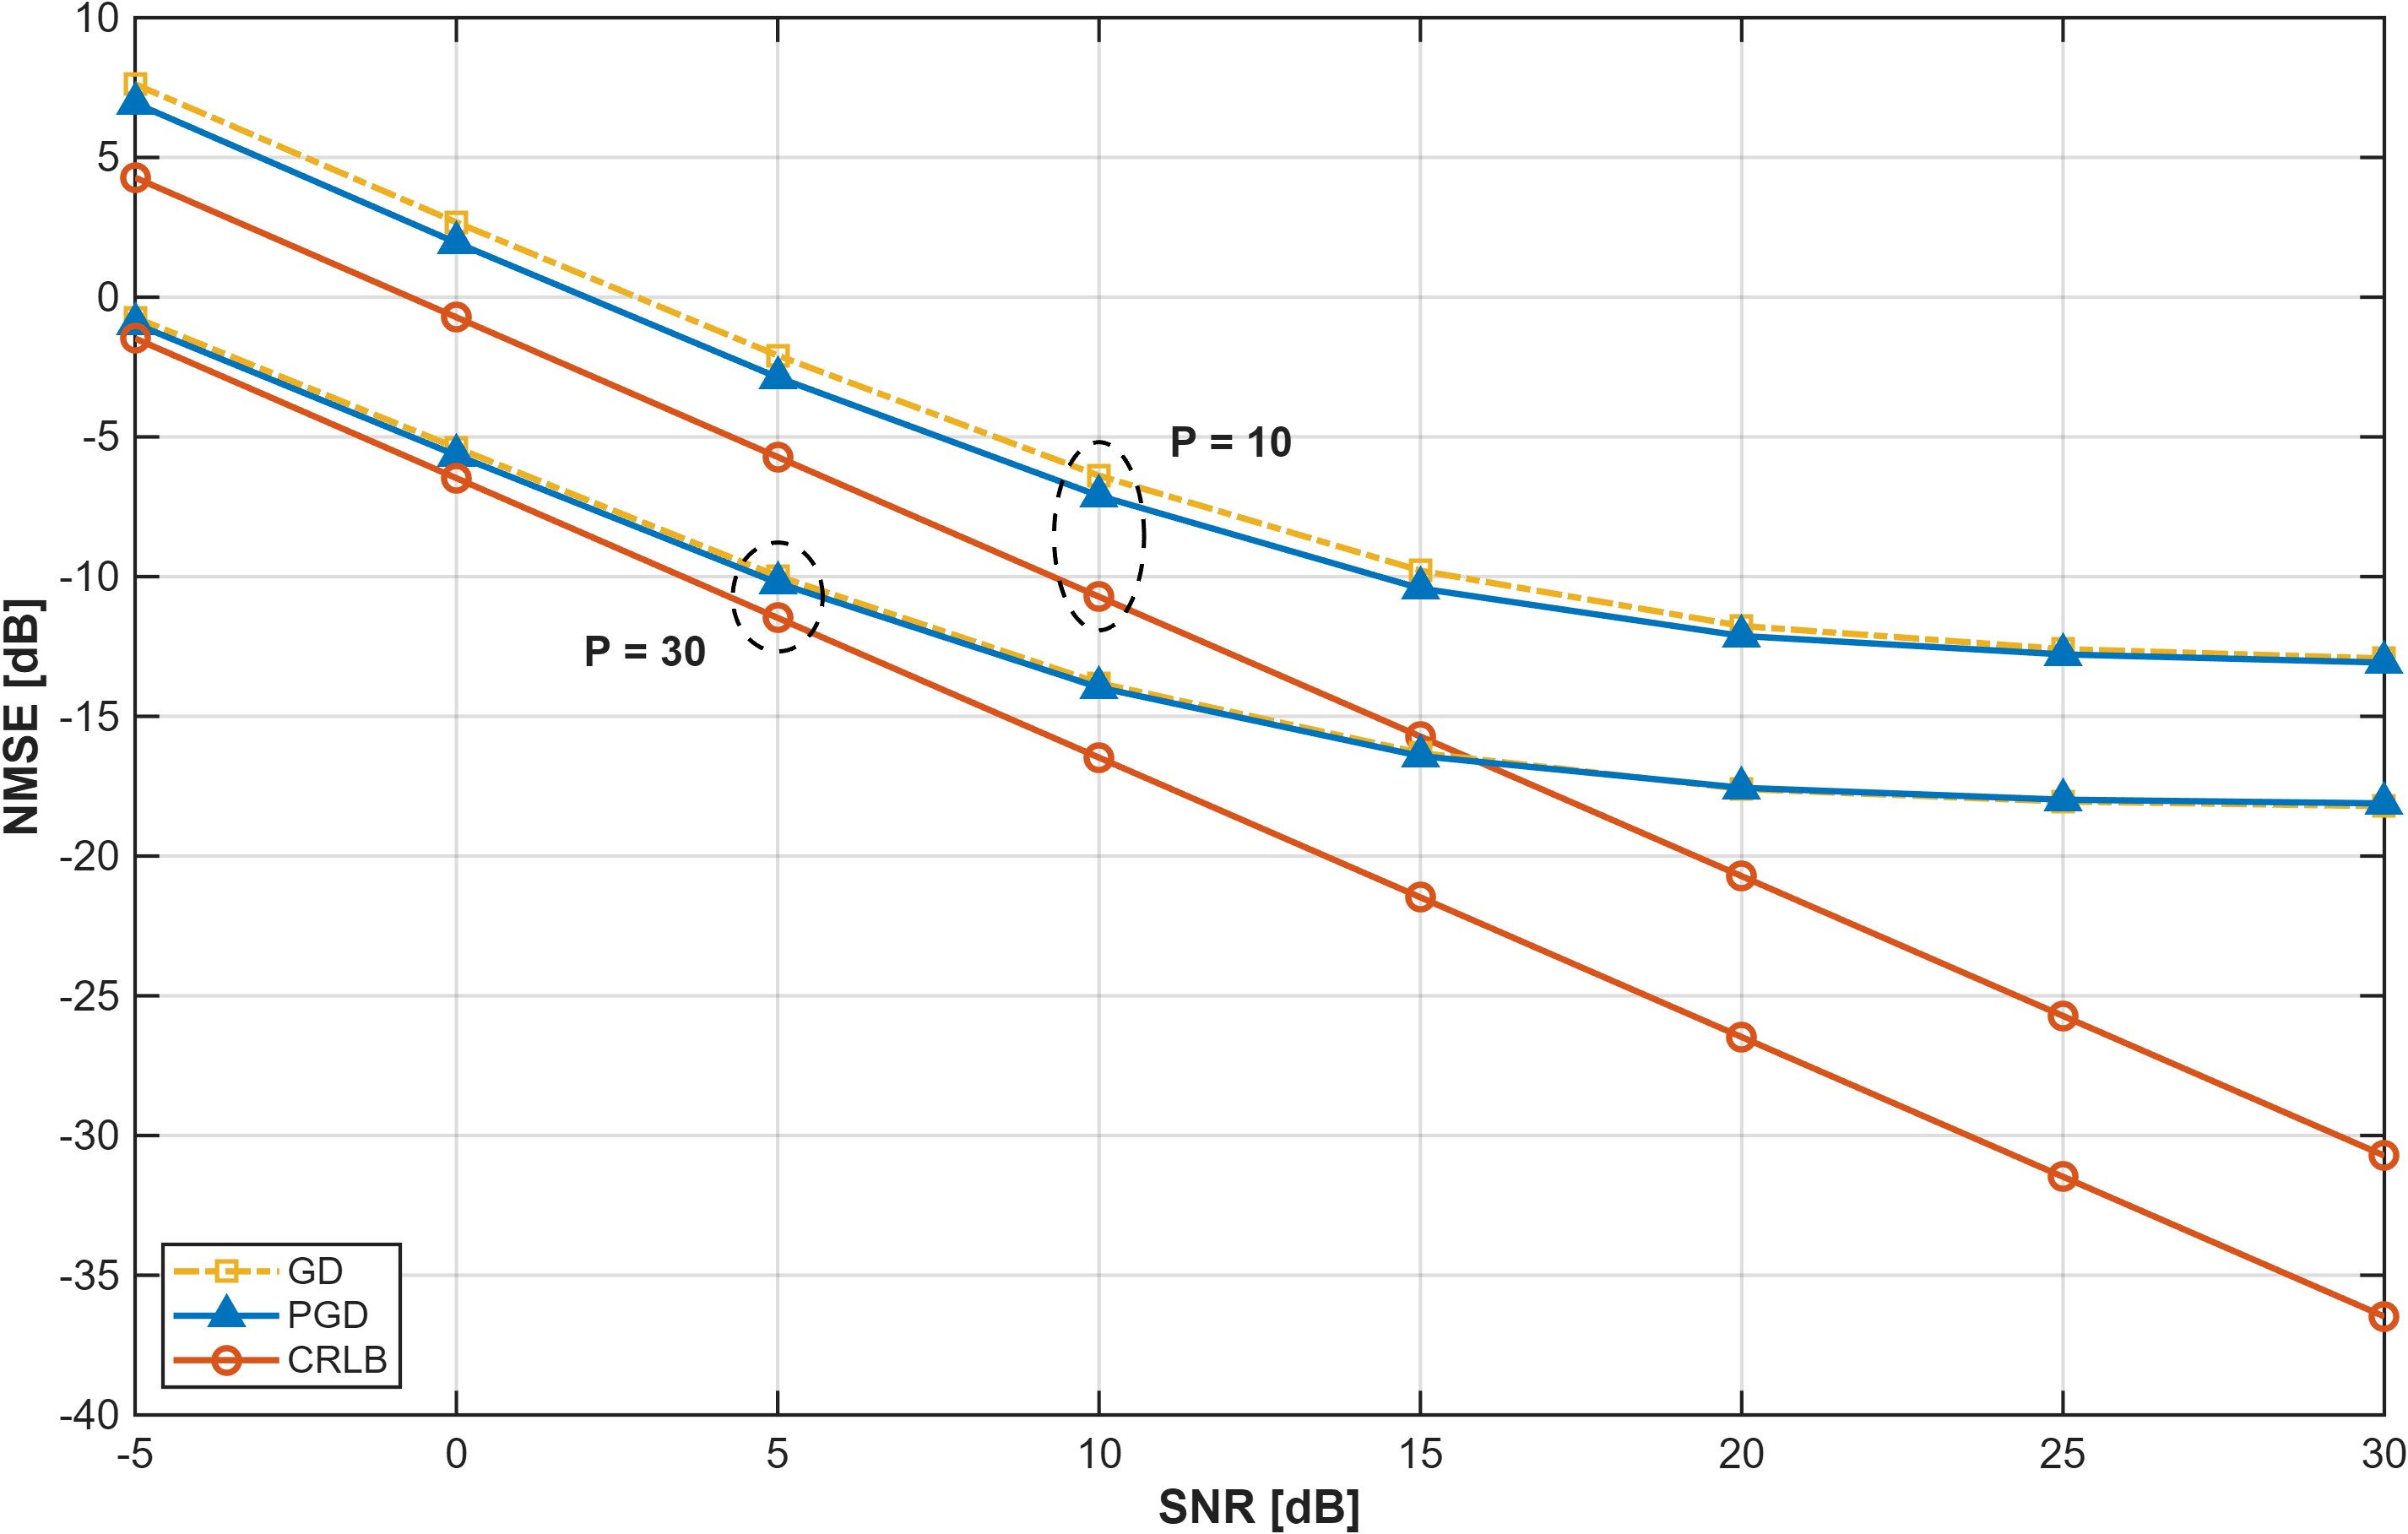
\includegraphics[width=0.75\textwidth]{ce_fig4_2d.png}
\caption{NMSE versus SNR for the $8\times8$ array: GD, PGD and CRLB.}
\label{fig:ce4}
\end{figure}

\noindent\textit{Effect of pilot length.} Figure~\ref{fig:ce5} shows the NMSE of PGD against the
number of pilots at 5~dB SNR.
\begin{itemize}[leftmargin=*,itemsep=2pt]
  \item The NMSE decreases steadily with $P$, since the CRLB is proportional to
        $(\mathbf S^*\mathbf S^T)^{-1}$, which shrinks as more pilots are added.
  \item With few pilots $\mathbf S^*\mathbf S^T$ is poorly conditioned and the estimate is noisier,
        so the gap from the CRLB is large: $5.8$~dB at $P=5$, $3.2$~dB at $P=10$ and $1.9$~dB at
        $P=15$.
  \item For $P\geq20$ the gap stays between $1.3$ and $1.7$~dB, which supports the conclusion of
        the paper that about 20 pilots are enough to get close to the bound.
\end{itemize}

\begin{figure}[H]
\centering
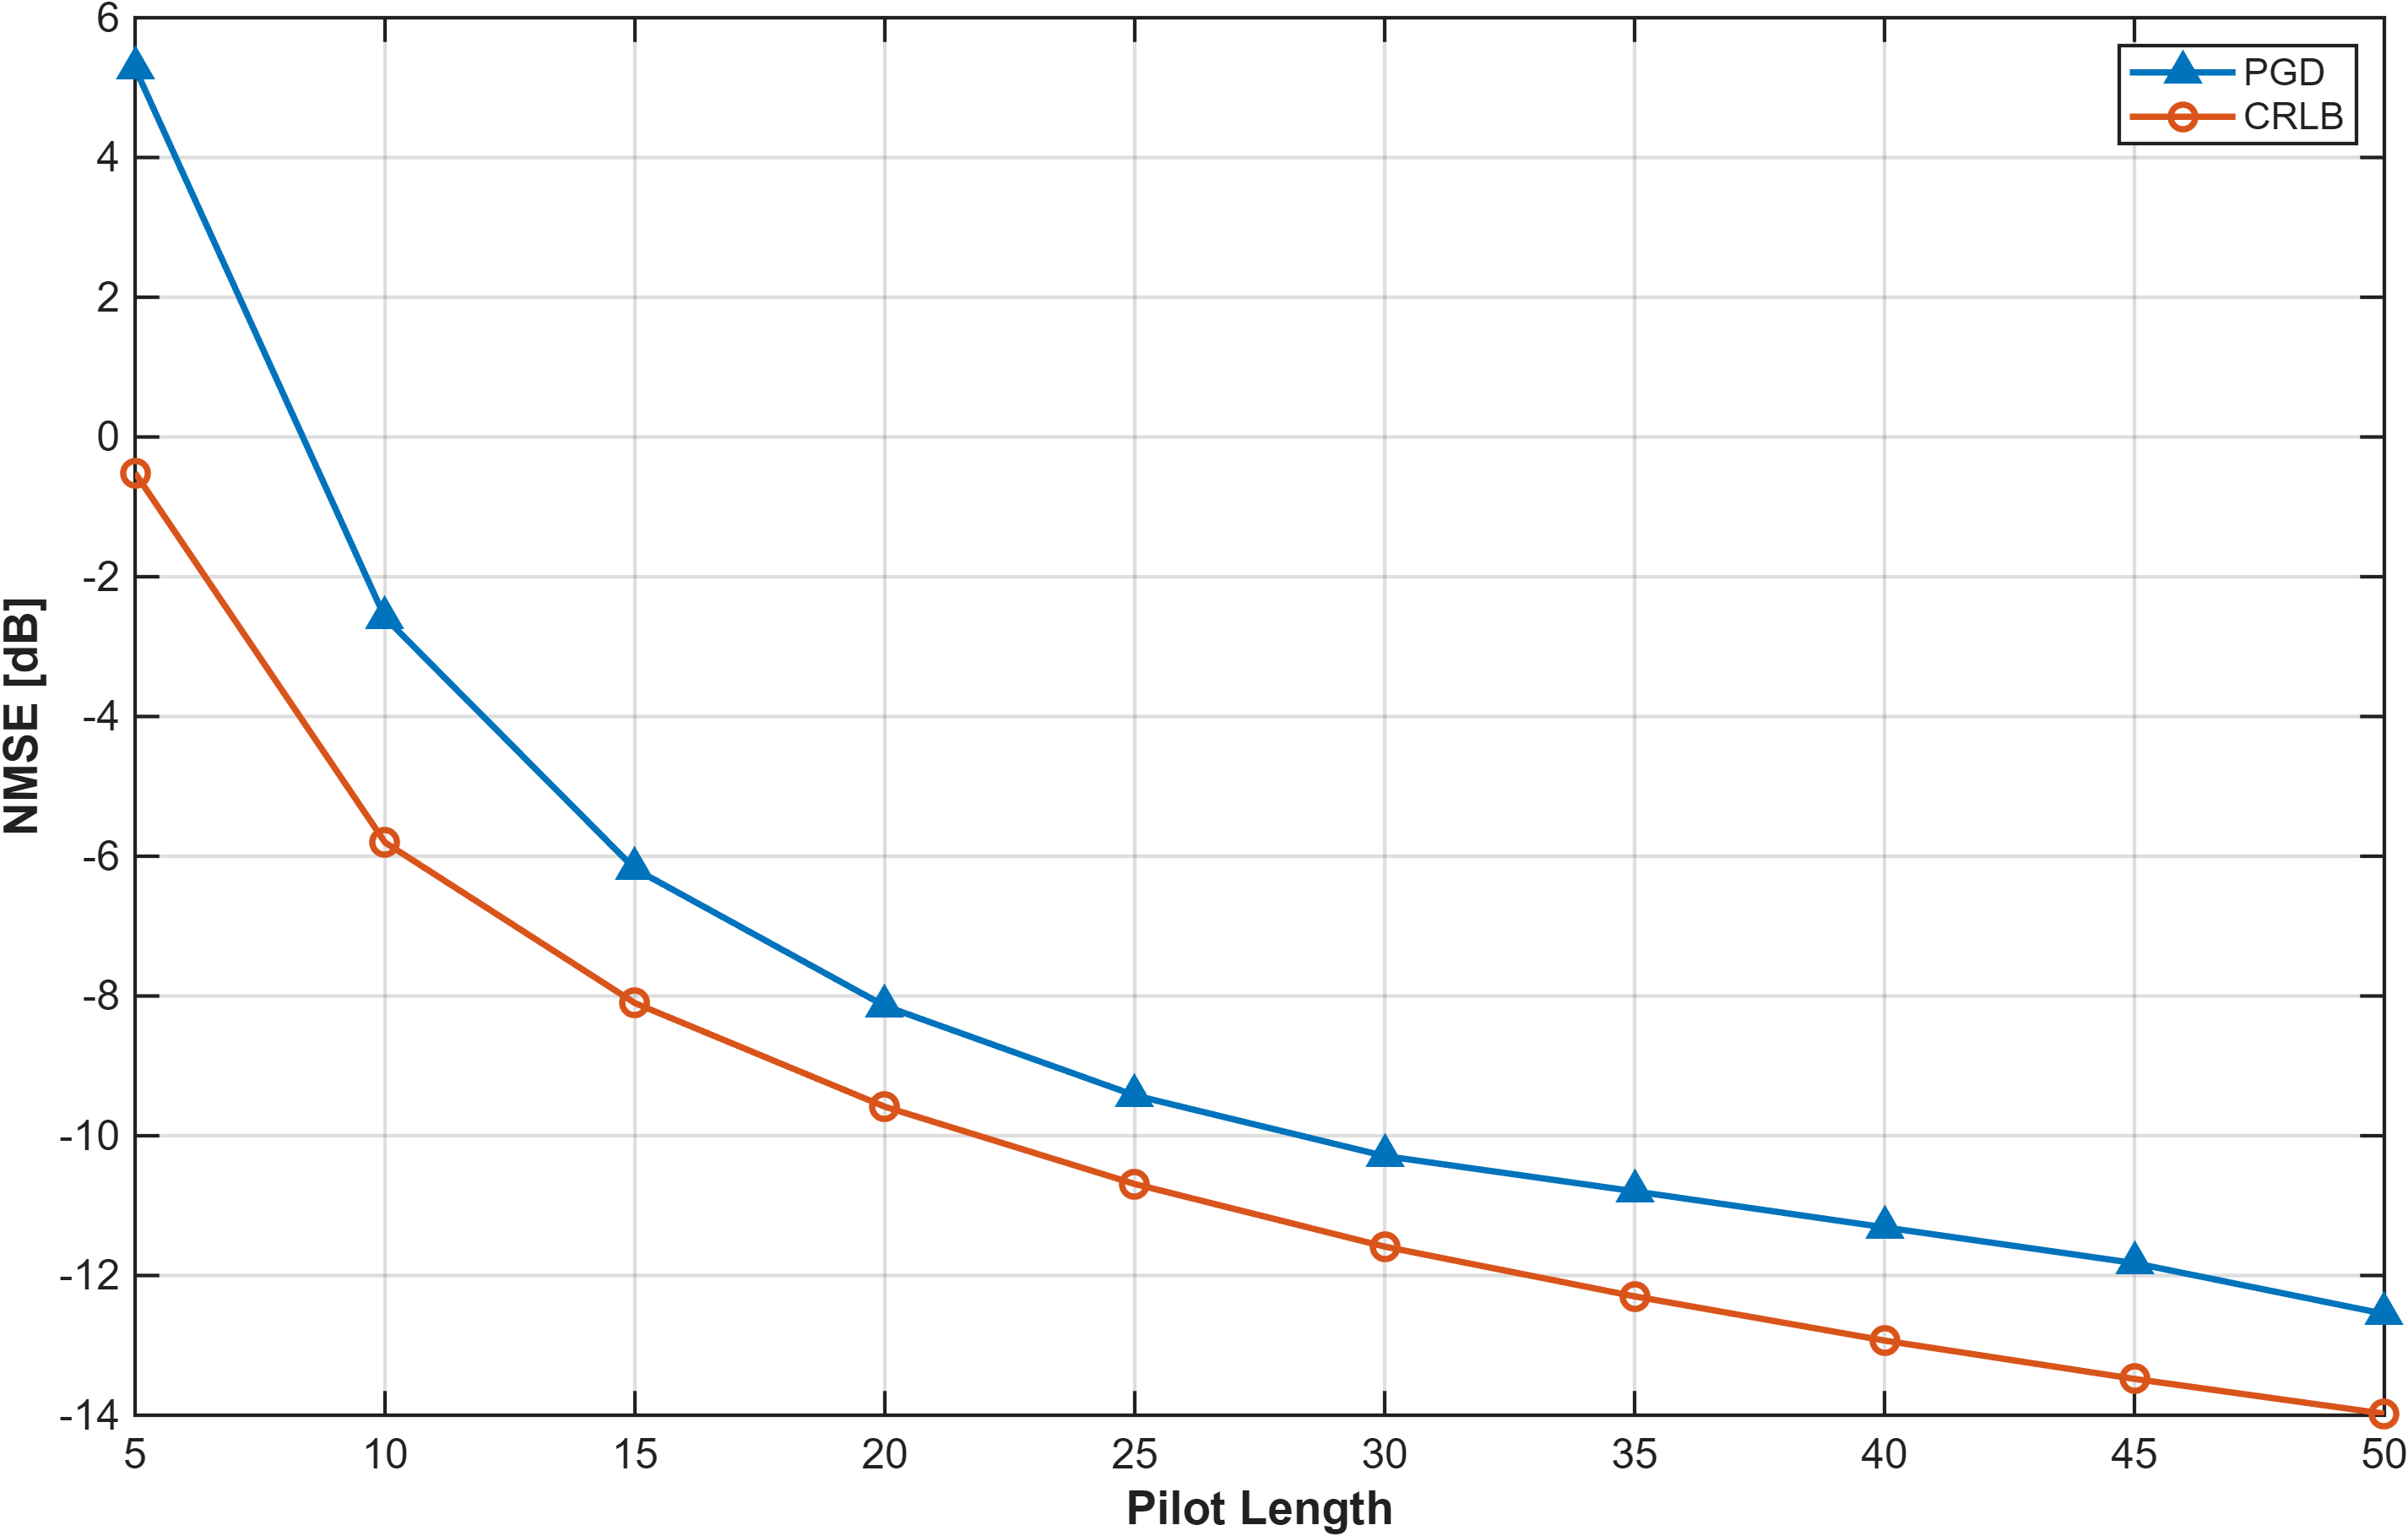
\includegraphics[width=0.75\textwidth]{ce_fig5_pilot.png}
\caption{NMSE versus pilot length for the $8\times8$ array at 5~dB SNR.}
\label{fig:ce5}
\end{figure}

% =========================================================
% 6. FINDINGS
% =========================================================

\section{Research Gaps}
\label{sec:findings}

The literature survey and the simulations point to the following limitations of the existing
work, which define the research gaps for the remaining part of the project.
\begin{enumerate}[leftmargin=*,itemsep=2pt]
  \item \textit{Single-antenna analysis of the LO-dressed receiver.} The LO-dressed receiver
        in~\cite{chen2025harnessing} is analysed only for a single antenna. Multi-antenna
        operation and channel estimation for an array of LO-dressed receivers, which measure
        both amplitude and phase, have not been studied.
  \item \textit{Two separate receiver models.} The LO-dressed mixer
        model~\cite{chen2025harnessing} and the magnitude-only phase-retrieval
        model~\cite{cui2025towards,xu2025channel} are developed independently, and no work
        compares or connects them.
  \item \textit{Dependence on a strong reference.} The estimators of~\cite{xu2025channel} rely on
        a first-order approximation that is valid only when $|b|\gg|a+n|$. As seen in
        Section~\ref{sec:impl2}, the linearisation error limits the NMSE at high SNR, and the
        behaviour of the estimators when the reference is not strong has not been studied.
  \item \textit{Structure not used in the exact model.} The biased GS
        algorithm~\cite{cui2025towards} works on the exact magnitude model but only for 1D arrays
        and without using the low-rank structure of the channel, while PGD~\cite{xu2025channel}
        uses this structure only in the linearised model.
  \item \textit{Limited use of learning-based methods.} The data-driven receiver
        of~\cite{liu2022deep} is evaluated only in terms of classification accuracy. Data-driven
        channel estimation for atomic MIMO receivers, compared against the CRLB, has not been
        explored.
\end{enumerate}

% =========================================================
% 7. FUTURE WORK
% =========================================================

\section{Future Work}
\label{sec:future}

\begin{enumerate}[leftmargin=*,itemsep=2pt]
  \item Study GS, EM-GS, GD and PGD for different reference-to-signal ratios, and find the bias
        of the linearised estimator when $|b|\gg|a+n|$ does not hold.
  \item Develop a channel estimator that does not depend on the first-order approximation, for
        example PGD on the exact magnitude model or an EM-based method that uses the rank
        structure, and compare it with the CRLB.
  \item Formulate channel estimation for an array of LO-dressed receivers, using the QuTiP
        response from Section~\ref{sec:impl1}, including its distortion region, as the
        measurement model.
  \item Explore machine learning and deep learning techniques for channel estimation in Rydberg
        atomic receivers, motivated by the data-driven approaches in~\cite{cui2026rare,liu2022deep},
        and compare their performance with the model-based estimators and the CRLB.
\end{enumerate}

% =========================================================
% REFERENCES
% =========================================================
\newpage
\begin{thebibliography}{99}

\bibitem{cui2026rare}
M.~Cui, Q.~Zeng, and K.~Huang, ``Rydberg atomic receiver: Next frontier of wireless
communications,'' \textit{arXiv:2412.12485v1}, Dec. 2024.

\bibitem{chen2025harnessing}
Y.~Chen, X.~Guo, C.~Yuen, Y.~Zhao, Y.~L.~Guan, C.~M.~S.~See, M.~Debbah, and L.~Hanzo,
``Harnessing Rydberg atomic receivers: From quantum physics to wireless communications,''
\textit{arXiv:2501.11842v1}, Jan. 2025.

\bibitem{cui2025towards}
M.~Cui, Q.~Zeng, and K.~Huang, ``Towards atomic MIMO receivers,'' \textit{IEEE J. Sel.
Areas Commun.}, vol.~43, no.~3, pp.~659--673, Mar. 2025.

\bibitem{xu2025channel}
B.~Xu, J.~Zhang, Z.~Chen, B.~Cheng, Z.~Liu, Y.-C.~Wu, and B.~Ai, ``Channel estimation for
Rydberg atomic receivers,'' \textit{IEEE Wireless Commun. Lett.}, vol.~14, no.~9,
pp.~2957--2961, Sep. 2025.

\bibitem{liu2022deep}
Z.-K.~Liu, L.-H.~Zhang, B.~Liu, Z.-Y.~Zhang, G.-C.~Guo, D.-S.~Ding, and B.-S.~Shi, ``Deep
learning enhanced Rydberg multifrequency microwave recognition,'' \textit{Nature Commun.},
vol.~13, Art. no.~1997, Apr. 2022.

\bibitem{sedlacek2012}
J.~A.~Sedlacek, A.~Schwettmann, H.~K\"ubler, R.~L\"ow, T.~Pfau, and J.~P.~Shaffer,
``Microwave electrometry with Rydberg atoms in a vapour cell using bright atomic
resonances,'' \textit{Nature Phys.}, vol.~8, no.~11, pp.~819--824, Nov. 2012.

\bibitem{jing2020}
M.~Jing \textit{et al.}, ``Atomic superheterodyne receiver based on microwave-dressed
Rydberg spectroscopy,'' \textit{Nature Phys.}, vol.~16, no.~9, pp.~911--915, 2020.

\bibitem{simons2019}
M.~T.~Simons, A.~H.~Haddab, J.~A.~Gordon, and C.~L.~Holloway, ``A Rydberg atom-based
mixer: Measuring the phase of a radio frequency wave,'' \textit{Appl. Phys. Lett.},
vol.~114, no.~11, Art. no.~114101, Mar. 2019.

\bibitem{netrapalli2015}
P.~Netrapalli, P.~Jain, and S.~Sanghavi, ``Phase retrieval using alternating
minimization,'' \textit{IEEE Trans. Signal Process.}, vol.~63, no.~18, pp.~4814--4826,
Sep. 2015.

\bibitem{johansson2012qutip}
J.~R.~Johansson, P.~D.~Nation, and F.~Nori, ``QuTiP: An open-source Python framework for the
dynamics of open quantum systems,'' \textit{Comput. Phys. Commun.}, vol.~183, no.~8,
pp.~1760--1772, 2012.

\end{thebibliography}

\end{document}
